% This file is part of the Apogee project.
% Copyright 2014 Melissa Ness and David W. Hogg.

% # short-term to-do
% - draft abstract
% - draft introduction

% # style notes
% - are they ``labels'' or ``labels''?  MKN:  Make a call and audit the whole text.
% - needs a name and to use it consistently as \thename

\documentclass[12pt, preprint]{aastex}
\usepackage{bm}
\input{vc}
\newcommand{\sectionname}{Section}
\newcommand{\documentname}{\textsl{Note}}

\newcommand{\set}[1]{\bm{#1}}
\newcommand{\mean}[1]{\overline{#1}}
\newcommand{\given}{\,|\,}
\newcommand{\teff}{\mbox{$\rm T_{eff}$}}
\newcommand{\feh}{\mbox{$\rm [Fe/H]$}}
\newcommand{\logg}{\mbox{$\rm \log g$}}
%\newcommand{\tc}{\fontfamily{qcr}\selectfont}
\newcommand{\tc}{\textsc{The Cannon}} 


 


\usepackage{morefloats}

\begin{document}

\title{\textsc{The Cannon:} Wavelength-independent stellar parameter determination using data-driven models}
\author{
  MKN,
  DWH,
  \&
  HWR}
\date{DRAFT / \gitdate\ / \githash\ / NOT FOR DISTRIBUTION}

% DWH say: Obey A&A abstract rules (ish).
%          They offer good guidance on abstract construction.


\begin{abstract}

Context: There are now numerous large programs to survey stars in the Milky Way, each of which is investing significant effort to determine and deliver stellar parameters and individual abundances across different wavelength regions. We present a generalised and wavelength independent regression technique to determine stellar parameters for large surveys, using a model built from data. Our approach does not require an intricate line-list characterisation at each new wavelength region observed by a survey, nor is it penalised by uncertainties in stellar models across different bands. With this methodology we effectively characterise how each pixel in a spectrum contributes to a given stellar parameter or label used to describe a star. In exploiting every pixel, we can determine stellar parameters at a fraction of the signal to noise compared to other techniques, for a given uncertainty. \\
Aims: We present \tc, our regression analysis approach to return labels for stars from large datasets, using data-driven models.  Our method transfers labels (of \teff, \logg\ and [Fe/H]) from a training set of data whose parameters are well determined (i.e. members of open and globular clusters) to the entire set of stars in a survey. Our work motivates the importance of having an established set of standard stars with well-determined labels. Given such standard calibrators, it is possible, via this technique of label-transfer, to place every stellar survey of the Milky Way on the same stellar parameter scale and homogeneously map the stellar population of the Milky Way from Northern and Southern hemispheres and using different wavelength regions. \\
Methods: We demonstrate \tc\ using the APOGEE dataset, to transfer labels from a training set of data of 19 open and globular clusters observed in APOGEE to every new star observed in the APOGEE DR10 data release. \\
Results:   We reproduce the stellar parameters for the APOGEE survey from DR10 and given the small intrinsic errors of this approach, can achieve this at a fraction (25\%) of the signal to noise required by minimisation techniques.   We obtain this performance via characterising the relationship between the labels of the stars in our training set and their flux, at each pixel. Our method is expandable to additional labels and relevant for chemical tagging.  Our work makes label determination of stellar spectra in large surveys accessible to the broader community and motivates the importance of having a ``gold standard'' set of stars studied at high resolution. \\



\end{abstract}

\section{Introduction}

There are numerous challenges in exploiting the large datasets of stellar spectra that have become available only in recent years. The first of these is the determination of stellar parameters which is typically a significant and iterative effort, customised specifically to the particular wavelength region of a given survey. The inputs to this procedure are a function of prior knowledge or assumptions about the wavelength region of interest and sensitive to uncertainties in this knowledge and in stellar models which are almost always explicitly relied upon. Typically, to determine stellar parameters, stellar models are used to derive a best-fit spectrum using some minimisation techqniue and a  post-calibration procedure is then applied, to set the results on an adopted physical scale across the parameter space. The inputs to these procedures, uncertainties and assumptions vary between surveys; this belies a second major challenge of the era of large datasets. \\

An optimal exploitation of all of these datasets relies on their homogenisation, i.e. a consistent stellar parameter scale for stars that have been observed by the Northern and Southern surveys, which operate across different wavelength regions. To facilitate this effort there is typically some cross over calibration stars observed between surveys. These may be stars studied and characterised at high resolution in the optical wavelength region and also globular and open clusters which have well determined labels. Rather than simply being used to post-calibrate surveys to a standardised physical scale, these calibration or standard stars afford a critical opportunity to create a data driven model.  This data driven model can be used for label-transfer (e.g. for labels of stellar parameters and individual abundances) from the calibration set to new stars in the survey. This relies on the parameter range and quality of the calibration set of stars, that they are observed between the different surveys and have a consistently defined standard set of labels. \\

In addition to the challenges, there are numerous opportunities in this era of large surveys of the Milky Way. These are not simply with respect to understanding more about the Galaxy itself, but for characterising the information in the data, building data driven models and implementing a differential analysis on large datasets. This can also identify where and how models diverge from data. We present a regression technique which demonstrates how a data driven model can be used to determine stellar parameters for the APOGEE survey, using label-transfer. However, our aim is distinct from simply determining parameters. We seek not to find the best fit spectra similarly to minimisation techniques but want to understand and characterise the spectra as a function of the labels which describe it.  We wish to determine, for each data point in our stellar spectra how the flux changes in response to the stellar labels. An outcome of this is that we produce a pipeline for stellar parameter determination for APOGEE spectra, which successfully reproduces the results from APOGEE DR10 and can perform a lower signal to noise for the same internal uncertainties compared to minimisation techniques. \\

We present in our paper this methodology of using label-transfer to efficiently and effectively determine stellar parameters for a large survey, using the example of the APOGEE survey but this method can be used for all stellar surveys. We demonstrate that by adopting a mathematical approach that exploits every pixel, the signal to noise required for at least the nominal stellar parameters is lower than minimisation methods. We quantify and describe how at each pixel in the APOGEE H-band stellar spectra, the flux varies with the labels. Our methodology is very relevant for chemical tagging in large datasets in the description and differentiation of the spectra on a mathematical basis which is inherent to the method; the characterisation of individual abundances themselves is likely insufficient to reconstruct stellar genealogy.  Our basic implementation of \tc\ that we present implements only three labels, but this can easily be extended to additional labels  (e.g. [$\alpha$/Fe], [X/Fe], age) and also more comprehensive models (e.g. Gaussian processes) , which we describe in Section X. %/lineage

We have adopted a bottom up approach for this project, starting with the most basic implementation and upgrading this iteratively. We firstly performed a proof of concept investigation, described in Section X. We then implemented \tc\ with a first order linear model, which we found to not  sufficiently describe the labels of the stars and so extended our model to quadratic form. The description of the training data and procedure we implement is in Section X. In Section X we describe and quantify how each of the pixels depends on the labels. In Section Y we present the results for \tc\ run through the APOGEE DR10 data. In section Y we make comparisons to APOGEE's pipeline ASPCAP for a few examples showing performance at lower SNR using single visit spectra. In Section Y we discuss addition of additional labels and future directions of this approach, moving to a more generalised model that will capture label-transfer outside of the input label parameter space. 



\section{Motivation}

- not convinced I want this in here let's see how it fits in by the end-of-draft stage

Preceding APOGEE, the IR spectral region has been sparsely studied and we therefore implemented some basic first tests to assess the sensitivity of the spectral features to changes in the stellar metallicity.  We identified a number of regions in APOGEE spectra that serve as relatively temperature and log g insensitive metallicity indicators over the parameter range of the calibrating stars. We found we could create an index to return an [Fe/H] for APOGEE spectra to an accuracy of $<$ 0.25 dex across the parameter range of the calibrators using only 25 $\AA$, which is about 1\% of the total spectral region. This index calibration is shown in Figure \ref{fig:index}.

\begin{figure}[h!]
  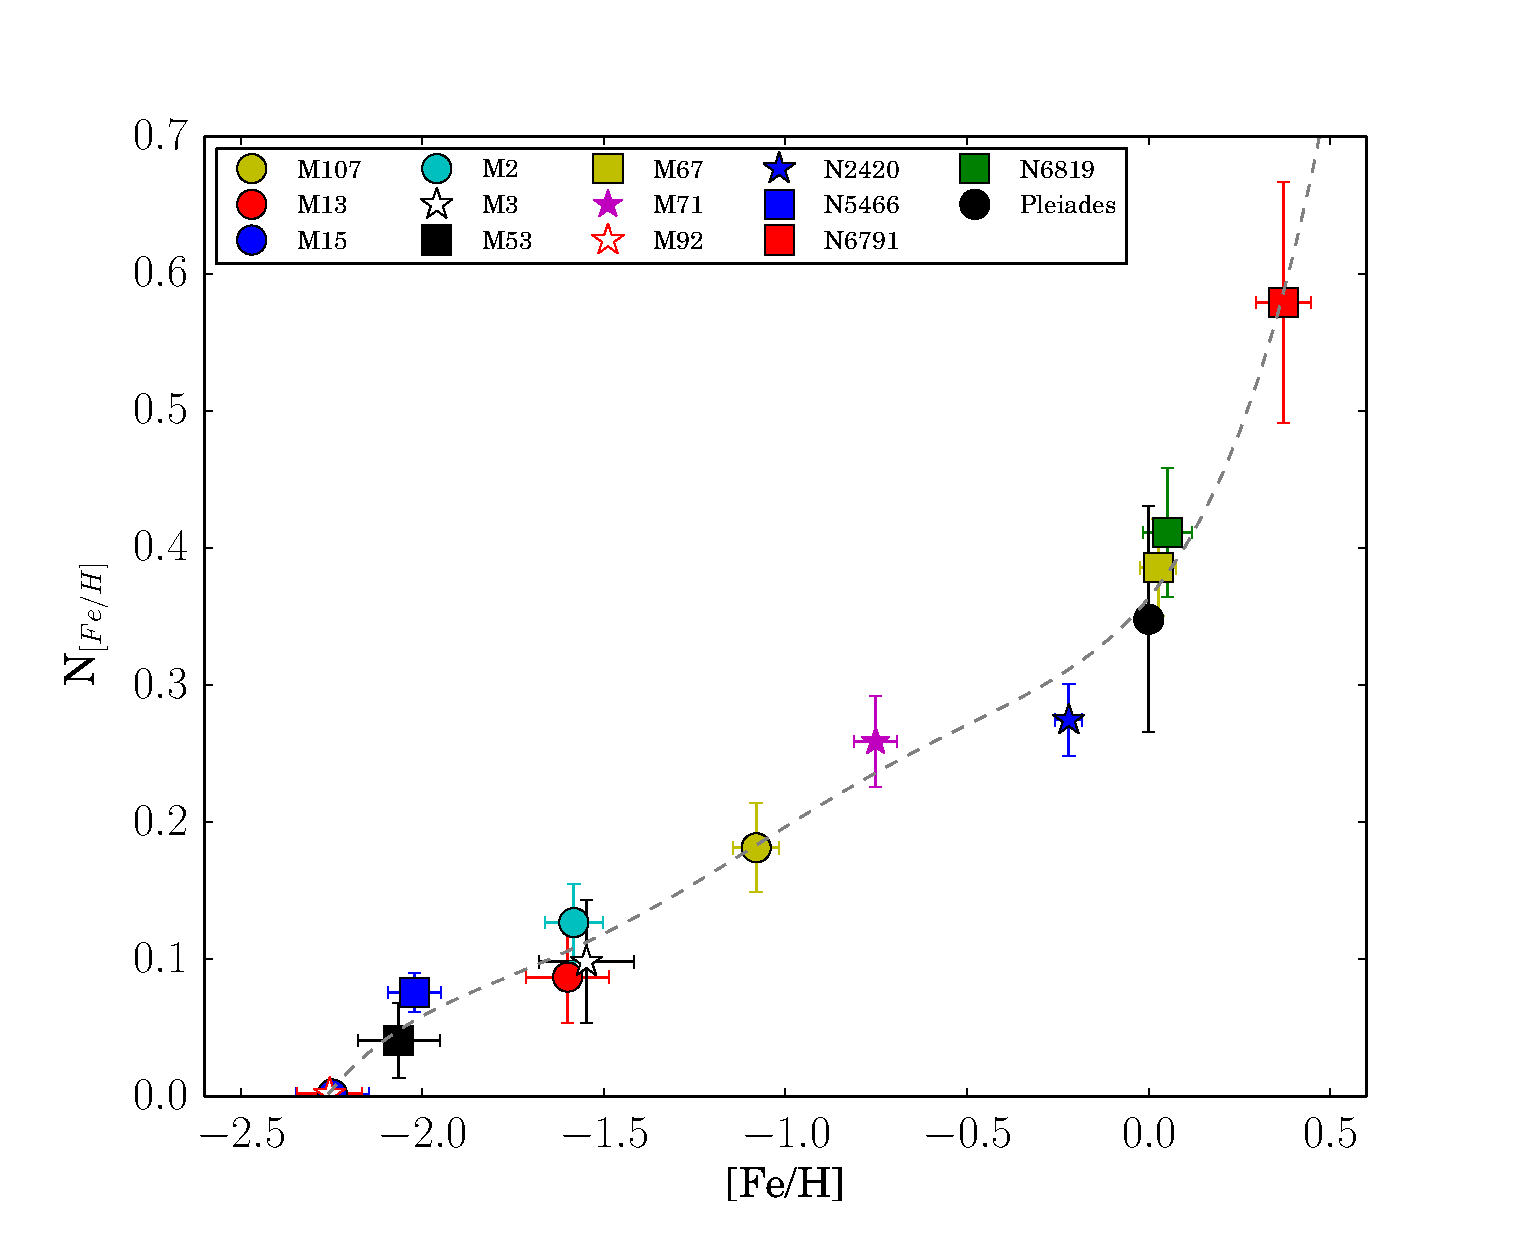
\includegraphics[width=\hsize]{./plots/metals_index.eps}
\caption{The calibration of metallicity of the clusters using an index N$_{[Fe/H]}$, derived from 30 $\AA$ (1\%) of the spectra, using 5 $\times$ lines determined to be [Fe/H]-sensitive and relatively \logg\ and \teff\ insensitive. The error bars represent the dispersion of the points
  around the mean. In total about 450  stars have been used for this
  calibration: M~107 (18 stars), M~13 (71 stars), M~15 (11 stars), M~2
  (19 stars), M~3 (73 stars), M~53 (16 stars), M~67 (24 stars), M~71
  (6 stars), M~92 (48 stars), NGC~2420 (9 stars), NGC~5466 (8 stars),
  NGC~6791 (23 stars), NGC~6819 (29 stars), and Pleiades (75 stars) }% \textbf{Note I am missing some clusters in this I should add them in} .}
\label{fig:index}
\end{figure}


From this first proof-of-concept phase, we implemented our regression analysis in pixel or line space, to determine the coefficients or spectral regions that might serve as stellar parameter indicators.  Ab initio we had the following aims: (i) to characterise the dependence of each pixel on the stellar parameters and identify the key regions of the spectra that are sensitive to the stellar parameters we wish to determine (Teff, log g, [Fe/H], [alpha/Fe]), (ii) use the fits to these regions (using calibration stars) as a baseline to derive the stellar parameters from any given APOGEE spectra and (iii) provide a tool to the community for implementation in the APOGEE-2 project + e.g. Hermes, where stellar parameters can be determined without explicit stellar models. Extensions of this include individual abundance labels and heuristic index determination which we investigate further in the discussion section.

\break 

\section{Data}

\subsection{Training Set Data}

The first step in the regression analysis implemented in \tc\ is to
obtain a training set.
This is a set of stars for which we have APOGEE spectra and
\emph{also} reliable stellar parameter estimates, both accurate and
precise (in as much as that is possible).
The training data are critical, as the output can only be as good as
the input training set, in the sense that if the training data are
wrong, the parameters output by \tc\ will be wrong in the same ways.
Also, because \tc\ may have to extrapolate to new parts of parameter
space as it encounters new kinds of spectra, the better the training
set covers the parameter space of interest (in \teff, \logg, [Fe/H],
[X/Fe], and so on), the less it has to perform uncertain
extrapolation.
The performance of a data-driven model like \tc\ can depend very
strongly on the size and quality of its training set.

For our purposes, an ideal training dataset may consist of members of
well studied open and globular clusters that have their stellar
parameter labels derived from high resolution spectral analysis in the
optical wavelength region.
In the optical region there is a significant legacy of stellar abundance analyses which employ clean, well defined lines with reliable oscillator strengths and take into account isotopic and hyperfine splitting effects for individual abundances. Furthermore, significant effort is currently underway with regard to the high resolution (UVES) analysis of a number of benchmark stars as part of the Gaia-ESO survey. These adopted ``standards'' would be ideal to include in any training set and supplement the open and globular cluster stars which are overt candidates, given their subsequent established labels (Joffre et al., 2014). %Significant effort is currently directed to updating line lists of clean unblended lines in the optical with reliable oscillator strengths and taking into account molecular isotopic splitting e.g. for Gaia-ESO (Heiter et al., in prep.).

The training set we employ for this data driven analysis is that of the globular and open cluster data observed by APOGEE for calibration of their abundance pipeline \citep{Meszaros2013}. This training data set is comprised of about 500 stars from 19 open and globular clusters, which span stellar parameter ranges of 3500 $<$ \teff\ $<$ 5300, 0 $<$ \logg\ $<$ 5 and --2.5 $<$ [Fe/H] $<$ 0.45. 

% note there are 20 in their list but 1 gc has only 1 star and the abundance looks incorrect to me. 

To place our output results from \tc\ on the APOGEE ASPCAP scale, we adopt the ``ASPCAP corrected'' stellar parameters for each of the stars in the training set as our labels for the stars. The corrections made by APOGEE for the cluster data are applied to the output of the ASPCAP pipeline which returns the initial parameters from comparisons to a library of stellar models. Temperature corrections are determined from the comparison the infrared flux temperatures of the stars \citep{Gonzalez2009}, \logg\ corrections are from the offset between ASCAP results and Kepler results for common stars and for [Fe/H] corrections are from the difference in the output of ASCAP compared the literature value of each cluster.  The APOGEE corrections that they determine in \citet{Meszaros2013} are valid only for stars with \logg\ $<$ 3.5 and are not implemented for the dwarfs. ASPCAP provides [M/H] values for these clusters, that are corrected to the [Fe/H] of the clusters and here we adopt this label as an [Fe/H]. This label from APOGEE does not explicitly use [Fe/H] lines, but this is derived from an [Fe/H] correction. The analysis in \citet{Meszaros2013} is restricted to giants and stars with SNR $>$ 70, determined to be the minimum for reliable stellar parameters by APOGEE. 

These corrections implemented by APOGEE in \teff\, \logg\, \feh\ place the giants in the cluster stars on or near the iscohrones (see Figures 7 and 8 in Meszaros et al., (2013)).  As there are no ASPCAP corrections implemented for the dwarf spectra, we instead determine temperatures for the dwarfs, which are all in the Pleaides, directly using same correction method as in \citet{Meszaros2013}. We determine the infrared flux temperature for the stars from \citep{Gonzalez2009} and apply a correction to the ASPCAP output based on the offset in the temperature scales. We find the following relation: $T_{\mbox{corrected}}$= 0.855*T$_{\mbox{ASPCAP}}$ + 1206.7. We do not attempt an individual metallicity correction for each dwarf star but rather set all [Fe/H] of the dwarf spectra to [Fe/H] = 0.03 (reference). To determine the log g for these dwarf stars, we shift the stars vertically to their nearest positions on an appropriate age-metallicity Padova isochrone (150 Myr at [Fe/H] = 0.03) \citep{Girardi2010}. Due to the high differential reddening to the Pleaides, and the subsequent large temperature errors using the IR flux method that result from this, we only selected the 64 from a total of 72 Pleiades dwarfs, eliminating those with high extinction of SFD E(J-K) $>$ 0.30.

Assuming the input labels from the ASPCAP corrected parameters determined from calibrations to literature cluster values also transfers the errors from the ASPCAP pipeline: of 150K in \teff\,  2 dex in \logg\ and 0.1 dex in \feh.   The uncertainties on the input labels will be included as an input parameter of the labels in future development stage of \tc\ and this may be particularly relevant when introducing multiple labels of individual elements, but for this initial demonstration we assume the input labels have no associated uncertainties. 



Adopting the labels from the ASPCAP output places \tc\ directly on the ASPCAP scale which is very instructive for comparison and analysis of the label-transfer method. We demonstrate excellent reproducibility of ASPCAP labels with our method, including at lower signal to noise than required by APOGEE (SNR $\ge$ 70). This is demonstrated in detail in Section X. We also return results for dwarfs in this method, however these are subject to the restriction that only $\sim$ 10\% of the stars in the training sample are dwarfs and all of these are at the same metallicity. Nevertheless, \tc\ is still able to differentiate dwarfs and giants and operates remarkably well given the constrained training set at \logg\ $>$ 3.5. 



%These results are shown in Section Y. \\


%Our method is calibrated across dwarfs and giants and can return reliable stellar parameters to a SNR of a fraction of this (30\%) XXX, with an intrinsic scatter of x,y,z in \teff, \logg, \feh. 


For comparison, we adopt a log g label for all of the training stars not from the Kepler scale, but rather take the \logg\ labels from the best vertical fits to the isochrone for the ages and metallicities for the clusters from the literature (with the temperatures fixed). We discuss our motivation for doing this and our results in the Discussion section of our paper.  In the following sections we compare the output on the HR digram for all DR10 stars of \tc\ versus ASPCAP for both calibration regimes and demonstrate that \tc\ reproduces APOGEE \teff\, \logg\, and \feh\ using a number of selected fields across the bulge, disk and halo with very small intrinsic errors, that are comparable to ASPCAP intrinsic errors at lower signal to noise than minimisation techniques. 

% the input labels and we demonstrate this in the section below.

% problems = dwarfs with emission but these go away with other model  

% and assume the metallicity of each star in the cluster is the same, at the mean metallicity of the cluster assuming the literature values of the cluster. We adopt a different literature value of M35(check) compared to APOGEE as this cluster appears to fit better at the value of XX according to the model and there is variation in the literature on this metallicity ranging from our adopted value of -0 35 to x. 

%We assume no errors on our labels for our input training set

\subsection{Flux Normalisation}

In fitting for labels that describe the spectra, we could in principle allow the continuum to be a label for which we can fit, in this way the continuum can be determined by the regression method. Alternatively, we can determine the continuum iteratively, but using the mean spectra determined from the training data. 

\section{Test Data} 

Our test data is the APOGEE continuum normalised DR10 spectra provided in the aspcapStar files (cite). These files provide continuum normalised multiple visit spectra with typical signal to noise of > 100. 

Describe what we do - continuum normalise in the exact same way as per the data. Then use the sigma to get the inverse variance of the data, critical in weighting for the regression in addition to the scatter parameter describing the standard deviation of the fit at every wavelength for all stars in the training set. This relies on the sigma array being correct. There are cases where does not capture bad flux, at 0 or other issues. This cases star is returned in non physical parameter space. Implemented own test to catch this by setting variance to a high value where flux is 0 or spiked and doing this for surrounding pixels as well. Also cases where absorption features in the spectra, use a chi2 metric to determine when star is far from fit. 


We do not use other flags but at end use other flags to see values in strange places - stars with large vscatter tend to lie between giant branch and dwarf branch. 

Additionally, syigma array does not capture this in the apStar files. 

There are bulge fields missing and these available in the apStar files, which are not flux normalised but we simply to this

For our SNR tests we need individual visits and therefore use the apStar files where are not flux normalised. 


Two pass - highly sensitive; temperature/SNR. 

\section{Discussion}

Although we find excellent agreement between \tc\ and ASPCAP by adopting ASCPAP corrected labels and additionally are able to derive parameters for dwarf stars in DR10, there are a number of issues with the output labels for the DR10 stars from \tc. The first is that for the HR diagram for all DR10 stars, which have been run though \tc, the giant branch is unphysically narrow. Furthermore, stars that have been determined using targeting flags and inspection of the spectra, to be dwarfs with chromospheric emission, lie in an unphysical space at very low [Fe/H] and \logg\ (see Figure X). The latter problem can be accounted for with additional tests on the stellar spectra to identify stars with chromospheric emission, however the narrowness of the giant branch is a consequence of the input labels of the training spectra. Tests on the input labels to \tc\ demonstrate that there is practically no difference to the output results from adopting individual [Fe/H] values for the stars (i.e. from the ASPCAP corrected values) or else a single [Fe/H] value for every star in a cluster, using the literature value of the cluster. 


The results using this alternative \logg\ calibration are in general mildly sensitive to the new adopted \logg\ training label. 
As the input labels are no longer on ASCAP corrected values, there are shifts from the ASPCAP scale in \logg\ with this new adopted input calibration. Cumulatively for running \tc\ through all DR10 stars, there are some more significant differences however.  The most dramatic difference is that the giant branch width from DR10 stars is consistent with the distribution in [Fe/H]. There is now excellent agreement with the isochrones for all DR10 to very low gravities, and fewer stars in unphysical regions. Furthermore, the stars with chromospheric emission which had previously unphysical values, with low \logg\ and \feh\, are output as dwarfs by the label transfer using the new model. 

\section{Spectral Model}

The model is that the observed, continuum-normalized spectrum, at each
wavelength, can be explained as a linear combination of real-valued
``labels'', or a linear combination of functions of those labels.
Here the labels will be things like effective temperature $\teff$,
logarithmic surface gravity $\logg$, and metallicity $\feh$.
Additionally, the model is that at each wavelength, the observed
spectrum will deviate from the linear combination by some additive
noise contribution, some of which comes from photon noise and
sky-subtraction noise and other instrumental contributions, and some
of which is an intrinsic scatter, presumed independent at each
wavelength.
The model is built using ``training data'' (with known labels) and then
used to tag (or infer labels for) the ``test data''.

In the training data there will be $N$ spectra $n$, each of which has
a continuum-normalized flux measurement $f_{n\lambda}$ at wavelength
$\lambda$, and an associated uncertainty variance
$\sigma_{n\lambda}^2$ from finite photon counts and instrumental effects.
If there are missing flux values in the training data, these can be
handled by setting variances to something very large (or inverse
variances to something very small).
Each of the training spectra $n$ has $K$ labels $l_{nk}$, each of which
is (for now) presumed to have negligible uncertainty.
The general model is
\begin{eqnarray}
f_{n\lambda} &=&
Y(\set{l}_n\given\set{\theta}_\lambda) + [s_\lambda^2 + \sigma_{n\lambda}^2]^{1/2}\,\xi_{n\lambda}
\label{eq:model}\\
\set{l}_n &\equiv& [l_{n1}, l_{n2}, \cdots, l_{nK}]
\quad,
\end{eqnarray}
Where $Y()$ is some (possibly complicated) function of the full set
of $K$ labels, $\set{l}_n$ is a vector or blob of the $K$ labels for spectrum $n$,
$\set{\theta}_\lambda$ is the set of parameters controlling the
function $Y()$ at each wavelength $\lambda$, $s_\lambda^2$ is an
intrinsic variance for the model at each wavelength and
$\xi_{n\lambda}$ is a Gaussian random number with zero mean and unit
variance.
That is, we have assumed that the noise is Gaussian, zero mean, and
independent for every measurement.
This model leads to the single-pixel log-likelihood function
\begin{eqnarray}
\ln p(f_{n\lambda}\given\set{\theta}_\lambda,s_\lambda^2) &=&
 -\frac{1}{2}\frac{[f_{n\lambda} - Y(\set{l}_n\given\set{\theta}_\lambda)]^2}{s_\lambda^2 + \sigma_{n\lambda}^2}
 -\frac{1}{2}\ln(s_\lambda^2 + \sigma_{n\lambda}^2)
 -\frac{1}{2}\ln 2\pi
\label{eq:like1}\\
\set{l}_n &\equiv& [l_{n1}, l_{n2}, \cdots, l_{nK}]
\quad.
\end{eqnarray}
Since all the spectra and pixels are treated as independent, each
wavelength $\lambda_\lambda$ can have its parameters
$[\set{\theta}_\lambda,s_\lambda^2]$ inferred independently, and all the
individual-spectra log-likelihoods can be added together to make
\begin{eqnarray}
\ln p(\set{f}_\lambda\given\set{\theta}_\lambda,s_\lambda^2) &=&
 \sum_{n=1}^N \ln p(y_{n\lambda}\given\set{\theta}_\lambda,s_\lambda^2)
\label{eq:like}\\
\set{f}_\lambda &\equiv& [y_{1\lambda}, y_{2\lambda}, \cdots, y_{N\lambda}]
\quad,
\end{eqnarray}
where $\set{f}_\lambda$ is the vector of spectral flux values for
the $N$ objects all at wavelength $\lambda$
We can set the parameters $[\set{\theta}_\lambda,s_\lambda^2]$ either by
optimizing the likelihood (\ref{eq:like}) or by applying priors and
performing some kind of probabilistic inference (with, say, Markov
Chain Monte Carlo techniques).
Here we will optimize for now.

In this \sectionname, we are treating the function parameters
$\set{\theta}_\lambda$ and the scatter $s_\lambda^2$ as free parameters, and the
labels $l_{nk}$ as fixed.
The likelihood function (\ref{eq:like}) is presented as being a
function of these free parameters.
In the next \sectionname, the tables will turn, and we will treat the
function parameters $\set{\theta}_\lambda$ and scatter $s_{\lambda}^2$ as fixed and
the labels $x_{nk}$ as parameters.
The difference is that here we are treating the training data as
having perfectly known labels, and later we will be inferring labels for
new spectra.

The simplest spectral model is that in which the functions $Y()$ are
linear in the labels:
\begin{eqnarray}
Y(\set{l}_n\given\set{\theta}_\lambda) &=&
 a_{\lambda 0} + \sum_{k=1}^K a_{\lambda k}\,[l_{nk} - \mean{l_k}]
\label{eq:linear}\\
\set{l}_n &\equiv& [l_{n1}, l_{n2}, \cdots, l_{nK}]
\\
\set{\theta}_\lambda &\equiv& [a_{\lambda 0}, a_{\lambda 1}, \cdots, a_{\lambda K}]
\quad ,
\end{eqnarray}
where the $a_{\lambda k}$ are linear coefficients, and
the $\mean{l_k}$ are offsets (possibly means of the training data) to
keep the model ``pivoting'' around a reasonable point in tag space.
This linear-in-labels form (\ref{eq:linear}) has many useful and
excellent properties.
The first is that optimization of the model, at fixed scatter
$s_\lambda^2$ is a pure linear-algebra operation (weighted least
squares); simultaneous optimization of all the parameters
$[\set{\theta}_\lambda,s_\lambda^2]$ is only nonlinear in the $s_\lambda^2$
parameter.
The second is that the tag inference (label-transfer; described in the
next Section) on the test data will have a very simple form.
The third is that the coefficients $a_{\lambda 0}$, seen as a discrete
function of wavelength $\lambda_\lambda$, can be seen as an estimate of
the \emph{mean spectrum} (provided that the offsets $\mean{x_k}$ are
the mean tag values over the $N$ training spectra); and the
coefficients $a_{\lambda k}$ can be seen as the mean first derivatives of
the expected spectrum with respect to each of the $k$ labels, estimated
over the range of the training data.

The results for the linear-in-labels model (\ref{eq:linear}) are shown
in Figures~XXX through YYY.  They show... departures from
linearity... outliers...

...what are we doing about outliers?  If anything?  Perhaps in discussion too...

- discuss how this method can be improved using priors as have this information e.g know space in Teff-logg that stars should lie in. 

...Of course weak lines might be closer to linear... what happens when
we restrict to weak lines?..

...is this a good model?  No; how do we know?

The (perhaps) second-simplest spectral model is that in which the
functions $Y()$ are quadratic in the labels:
\begin{eqnarray}
Y(\set{l}_n\given\set{\theta}_\lambda) &=&
 a_{\lambda 0} + \sum_{k=1}^K a_{\lambda k}\,[l_{nk} - \mean{l_k}]
 + \sum_{k=1}^K \sum_{k'=k}^K a_{\lambda kk'}\,[l_{nk} - \mean{l_k}]\,[l_{nk'} - \mean{l_{k'}}]
\label{eq:quadratic}\\
\set{l}_n &\equiv& [l_{n1}, l_{n2}, \cdots, l_{nK}]
\\
\set{\theta}_\lambda &\equiv& [a_{\lambda 0}, a_{\lambda 1}, \cdots, a_{\lambda K},
                            a_{\lambda 11}, a_{\lambda 12}, \cdots, a_{\lambda KK}]
\quad ,
\end{eqnarray}
where the $a_{\lambda k}$ and $a_{\lambda kk'}$ are linear coefficients, and
the $\mean{l_k}$ are offsets (possibly means of the training data) to
keep the model ``pivoting'' around a reasonable point in tag space.
This quadratic-in-labels form (\ref{eq:quadratic}) is similar to and
different from the linear-in-labels form (\ref{eq:linear}) in a number
of ways.
It is still the case that optimization of the model, at fixed scatter
$s_\lambda^2$ is a pure linear-algebra operation (weighted least
squares).
However, tag inference (described in the next Section) on the test
data will no longer be simple; it will now require non-linear
optimization.
The coefficients $a_{\lambda 0}$ can still be seen as an estimate of the
\emph{mean spectrum} (provided that the offsets $\mean{l_k}$ are the
mean tag values); the first-order coefficients $a_{\lambda k}$ can still
be seen as first derivatives of the expected spectrum with respect to
each of the $k$ labels, but now evaluated at the mean spectrum; the
second-order coefficients $a_{\lambda kk'}$ can now be seen as mean
second derivatives of the expected spectrum with respect to pairs of
labels $k$ and $k'$.

The results for the quadratic-in-labels model (\ref{eq:linear}) are shown
in Figures~XXX through YYY.  They show... departures from
linearity... outliers... is it really a better model?..

\section{Hans-Walter nomeclamenture}

- David can you help me reconcile yours with HW's i.e. compromise/put in both somehow...svp?...

Step 1. \\

We want to firstly determine the coefficients of the fit of the training data given their labels, given s = 1..N$_spectra$, \lambda = 1 to N$_pixels$ and labels l = 1 to N$_labels$. There is a coefficient at every pixel, 
${\left \vector{\theta_\lambda} \right}_lambda$ and there is a set of labels for every star, ${\left \vector{\theta_s} \right}_s$. Given a flux for every star in the training spectra at every wavelength, 
\begin{equation}
f_{\lambda s}(\vector{c_\lambda}\vector{l_s}) = mean(f_\lambda) + dot( \vector{\theta}   {L^'}_s (\vector{l_s})  ) 
\end{equation}

where {L^'}_s = f(\vector{L_s}, order) so for linear \tilde{L_s} = \vector{L_s} and for quadratic 
\tilde{L_s} = \matrix{}

Getting the coefficients wavelength-by-wavelength from all of the training spectra: 

\begin{eqnarray}
\ln p(\set{data}_\lambda\given\set{\vector{l_s}}, {\vector{\theta}}_\lambda,\sigma_\lambda) &=&
- \sum_{s=1}^N_{spec} \divide{(f_{\lambda}_s - \mean(f_\lambda} -  dot( \vector{\theta_\lambda}^T, \vector{l_s} }^2{2(\delta_\lambda_s + \sigma{^2}_\lambda)}
\end{eqnarray}
where \delta is the pixel uncertainty, from the instrument and from the shot noise and \sigma is the scatter of the fit. So optimise to get the coefficients and the scatter parameters, $\vector{\theta_\lambda}$, $\sigma_\lambda$, for known labels \vector{l_s} in the training set. 

Step 2: 

Optimise the sample solving for the labels \vector{l_s} given the set of coefficients and scatters for those coefficient fits, 
$\left c_\lambda \right_{\lambda}$. 

Here: \\
\begin{eqnarray}
\ln p(\set{data}_\s\given\set{\vector{l_s}}, ({\vector{\theta_{\lambda}}})_\lambda,({\sigma_\lambda})_\lambda) &=&
- \sum_{s=1}^N_{pixels} \divide{(f_{\lambda}_s - \mean(f_\lambda} -  dot( \vector{\theta_\lambda}^T, \vector{l_s} }^2{2(\delta_\lambda_s + \sigma{^2}_\lambda)}
\end{eqnarray}

This time optimise the function solving for the labels \vector{l_s} given the set of coefficients at every wavelength $\left \theta_\lambda $right _\$lambda$ determined from the training set. \\


\section{Parameter estimation}

In the previous \sectionname, we built data-driven spectral models
from training data.
These models have the property that, given labels, they can be used to
predict continuum-normalized flux, up to observational and intrinsic
scatter.
In this \sectionname, we are going to solve the inverse problem; we
are going to presume that we have spectra, but we don't have labels.
In this case, we will use inference to obtain labels for the untagged
spectra.
These untagged spectra will be referred to as the ``test data'' in
what follows.

In the test data there will be $M$ spectra $m$, each of which---as in
the training data---has a continuum-normalized flux measurement
$y_{m\lambda}$ at each of $L$ wavelengths $\lambda_\lambda$, and an
associated observational uncertainty variance $\sigma_{m\lambda}^2$.
Again, if there are missing flux values in the test data, these can be
handled by setting variances to something very large.
The difference between the training data and the test data is that the
test data do not (yet) have known labels $x_{mk}$; we are going to infer
these.

Just as in the previous \sectionname, our model is given in
equation~(\ref{eq:model}).
This model leads to the same likelihood function given in
equations~(\ref{eq:like1}) and (\ref{eq:like}), but this time seen as
being functions not of the function parameters $\set{\theta}_\lambda$ and
scatter $s_\lambda^2$ but instead as functions of the \emph{labels}
$x_{mk}$:
\begin{eqnarray}
\ln p(y_{m\lambda}\given\set{x}_m) &=&
 -\frac{1}{2}\frac{[y_{m\lambda} - Y(\set{x}_m\given\set{\theta}_\lambda)]^2}{s_\lambda^2 + \sigma_{m\lambda}^2}
 -\frac{1}{2}\ln(s_\lambda^2 + \sigma_{m\lambda}^2)
 -\frac{1}{2}\ln 2\pi
\\
\ln p(\set{y}_m\given\set{x}_m) &=&
 \sum_{\lambda=1}^L \ln p(y_{m\lambda}\given\set{x}_m)
\label{eq:taglike}\\
\set{x}_m &\equiv& [x_{m1}, x_{m2}, \cdots, x_{mK}]
\\
\set{y}_m &\equiv& [y_{m1}, y_{m2}, \cdots, y_{mL}]
\quad,
\end{eqnarray}
where the likelihood functions are given as a function of labels now,
the sum is now over the full set of $L$ wavelengths
$\lambda_\lambda$, and the vector $\set{y}_m$ is the vector of fluxes from
spectrum $m$ for all $L$ wavelengths $\lambda_\lambda$.
These likelihood functions effectively assume that the function
parameters $\set{\theta}_\lambda$ and scatters $s_\lambda^2$ are all known (from
the training data).
New labels $x_{mk}$ for object $m$ can be obtained either by maximizing
the likelihood function (\ref{eq:taglike}), or else by applying priors
and performing probabilistic inference.
Here we will optimize for now.

When we use the simple linear-in-labels form (\ref{eq:linear}) for the
mean model $Y()$, the optimization to obtain maximum-likelihood labels
(given parameters $[\set{\theta}_\lambda, s_\lambda^2]$) is simple linear
least-square fitting.
This optimization is obtained by straightforward linear algebra on the
spectral pixels $y_{m\lambda}$, and standard frequentist confidence
intervals can be obtained similarly.
Results for the linear-in-labels model are shown in Figures~XXX through
YYY.

When we use the quadratic-in-labels form (\ref{eq:quadratic}) for the
mean model $Y()$, there is no simple linear-algebra operation that
optimizes the likelihood.



...why is linear so much easier than quadratic or GP?  Methodological details

...leave-one-cluster-out cross-validation

...application to some example APOGEE targets and comparison to ASPCAP




\section{Results}

We firstly demonstrate the results for \tc\ compared with those of ASPCAP for three selected fields, in the disk, bulge and halo. 

We find lesser agreement in fields in the plane where APOGEE targets cool supergiant stars. We eliminated the possibility that our results were being degraded by diffuse interstellar bands \citep{Ziaskowski2014} by creating a mask to eliminate this region in training. However, APOGEE results are uncertain for cool temperature stars \teff\ $\sim$ 3500 K so this may be the source of the discrepancy. Alternatively, we have no training data at the lowest temperatures of stars targeted in the plane, so our model may not be able to capture the labels for these stars. Indeed the $\chi^2$ evaluation of the model fit demonstrates at the extent of the training set, the largest $\chi^2$ values are returned for the stars, which makes sense give the labels extend beyond the boundaries of the model and are an extrapolation. 

We show \tc\ - APSCAP comparison for three bulge, disk and halo fields in Figures X - Y, with their corresponding $\chi^2$ fits. These are typical comparisons for all of the fields except in the plane where there are more cool stars due to targeting. The mean bias, offset and precision from \tc\ for the stars in these fields is shown in these figures. 



\begin{figure}[h!]
  \includegraphics[width=\hsize]{./plots/DR10_isochrone_mknA.png}
\caption{\small{}}
\label{fig:cal}
\end{figure}

\begin{figure}[h!]
  \includegraphics[width=\hsize]{./plots/density_mknA.png}
\caption{\small{}}
\label{fig:cal}
\end{figure}


\section{Performance at a fraction of the SNR} 

- intrinsic errors are small 
- therefore get errors on the order of X,Y,Z with SNR of not 100 but 25 - as using information in all of spectrum. 

Example of field run thourgh with only one exposure and not many. 



\section{Anomalous Spectra}

- blue plume is young dwarf stars with chromospheric emission
- also stars in intermediate area - also placed there by ASPCAP - unclear currently what these are : binaries? perhaps - mean of the two. also very unequal training set. 

- See Figure X for the training set histograms of t, g, feh. 

For our regression analysis, where pixels are directly compared between stars in the training set, it is essential to have a robust continuum normalisation that will ensure pixels are compared fairly between stars of different parameters. We therefore implement a weighted median method, but instead of returning the central tendency we consider the 85\% quantile, returning the typical continuum level and effectively excluding outliers, considered over intervals of 50\AA of the spectra. This provides a consistent normalisation across the spectra. Three typical spectra are shown in Figure X demonstrating this normalisation routine is effective. Similarly to the training set, all data input to the regression must be treated in the same way with the same continuum normalisation.
\textit{ note - need to consider coolest stars and also high signal to noise and may need to adjust quantile for this. }

re-continuum-normalize; how?

demonstrate that the normalization is good.

meta-data on cluster stars; why do we believe it; table - just reference Meszaros 2013 for this or we are repeating information. 

...We need a plot that shows \teff\ vs \logg\ colored by \feh\ for the training stars!

%read in data; which files, etc.
%
%A training dataset may ideally be one that consists of a set of stars that extend over the parameter range of the observations, in \teff\, \logg\, [Fe/H], [X/Fe] and have their labels derived from high resolution spectral analysis in the optical, where abundance analyses can employ reliable and clean well defined lines and take into account isotopic and hyperfine splitting effects for individual abundances. The training set we employ for this data driven analysis is that of the globular and open cluster data observed by APOGEE for calibration of their abundance pipeline \citep{Mesaroz2013}. This training data set is comprised of 20 open and globular clusters, which span stellar parameter ranges of 3500 $<$ \teff\ $<$ 5300, 0 $<$ \logg 5 and --2.5 $<$ [Fe/H] $<$ 0.45. We adopt the ``ASPCAP corrected'' stellar parameters of each of these stars in the training set as our labels for the stars; this nominally ensures that we are on the same calibration as APOGEE for stellar parameters. The corrections made by APOGEE for the cluster data are applied to the direct output of the ASPCAP pipeline based on a temperature calibration to the infrared flux method \citep{Gonzalez2009} ,a \logg\ correction from the offset between ASCAP results and Kepler results for common stars and [Fe/H] offsets from the output of ASCAP versus the literature value of each cluster.  The APOGEE corrections that they determine are valid only for stars with \logg\ $<$ 3.5 and are not implemented for the dwarfs. 
%
%These corrections place the giants in the cluster stars on or near the iscohrones (see Figures 7 and 8 in Meszaros et al., (2013)). We  also correct the ASPCAP dwarf cluster spectra to the infrared flux value of \citep{Gonzalez2009} which is small at their temperatures, offset the metallicities of these stars by the difference between the mean value from the ASPCAP pipeline and the literature values of the clusters from Meszaros et al., 2013 and shift the \logg\ values of the stars to their nearest positions on the isochrone, moving the stars vertically without adjusting the other calibrated parameters. \textit{actually I have not done this yet - most important will be logg other changes are small}.
%
%The analysis in \citet{Meszaros2013} is restricted to giants and stars with SNR $>$ 70, determined to be the minimum for reliable stellar parameters. Our method is calibrated across dwarfs and giants and can return reliable stellar parameters to a SNR of XXX, with an intrinsic scatter of x,y,z in \teff, \logg, \feh. 
%
%- See Figure X for the training set histograms of t, g, feh. 
%
%For our regression analysis, where pixels are directly compared between stars in the training set, it is essential to have a robust continuum normalisation that will ensure pixels are compared fairly between stars of different parameters. We therefore implement a weighted median method, but instead of returning the central tendency we consider the 85\% quantile, returning the typical continuum level and effectively excluding outliers, considered over intervals of 50\AA of the spectra. This provides a consistent normalisation across the spectra. Three typical spectra are shown in Figure X demonstrating this normalisation routine is effective. Similarly to the training set, all data input to the regression must be treated in the same way with the same continuum normalisation.
%\textit{ note - need to consider coolest stars and also high signal to noise and may need to adjust quantile for this. }
%
%re-continuum-normalize; how?
%
%demonstrate that the normalization is good.
%
%meta-data on cluster stars; why do we believe it; table - just reference Meszaros 2013 for this or we are repeating information. 
%
%...We need a plot that shows \teff\ vs \logg\ colored by \feh\ for the training stars!


\section{Discussion}

...Did it work and etc?  Weak lines, order, etc.

...Structure of the problem:
We \emph{didn't} do the standard machine-learning thing of ``just'' asking the fluxes to predict the labels.
We asked the labels to predict the fluxes, and then once that worked, we found the labels that predict the fluxes for other stars.
This structure permits us to respect the noise model (noisy, heteroskedastic fluxes).

...Limitations of the training sample.  Mainly its smallness!

...Limitations of assuming the training sample has perfect labels.

...Linear (or quadratic) model is a very rigid assumption; obviously wrong.
Generalize to a GP at every wavelength.

...Limitations of working at one wavelength at a time in model-building.

...Limitations of the inference procedure at tagging time

...What would the fully probabilistic generalization look like?
It would involve generating samples of $[\set{\theta}_\lambda, s_\lambda^2]$ at each wavelength $\lambda_\lambda$ at training time.
Then using all these samples at tagging time.
Produce also a sampling of labels $\set{x}_m$ for each object $m$.
Would have the great advantage that we could use partially or noisily tagged objects in training!
Would be equivalent to fitting everything simultaneously (that is, training and tagging at the same time).
Would require priors on everything.

...Next-generation applications of these methods, esp chemical tagging

\section{Draft Figures}



\begin{figure}[h!]
  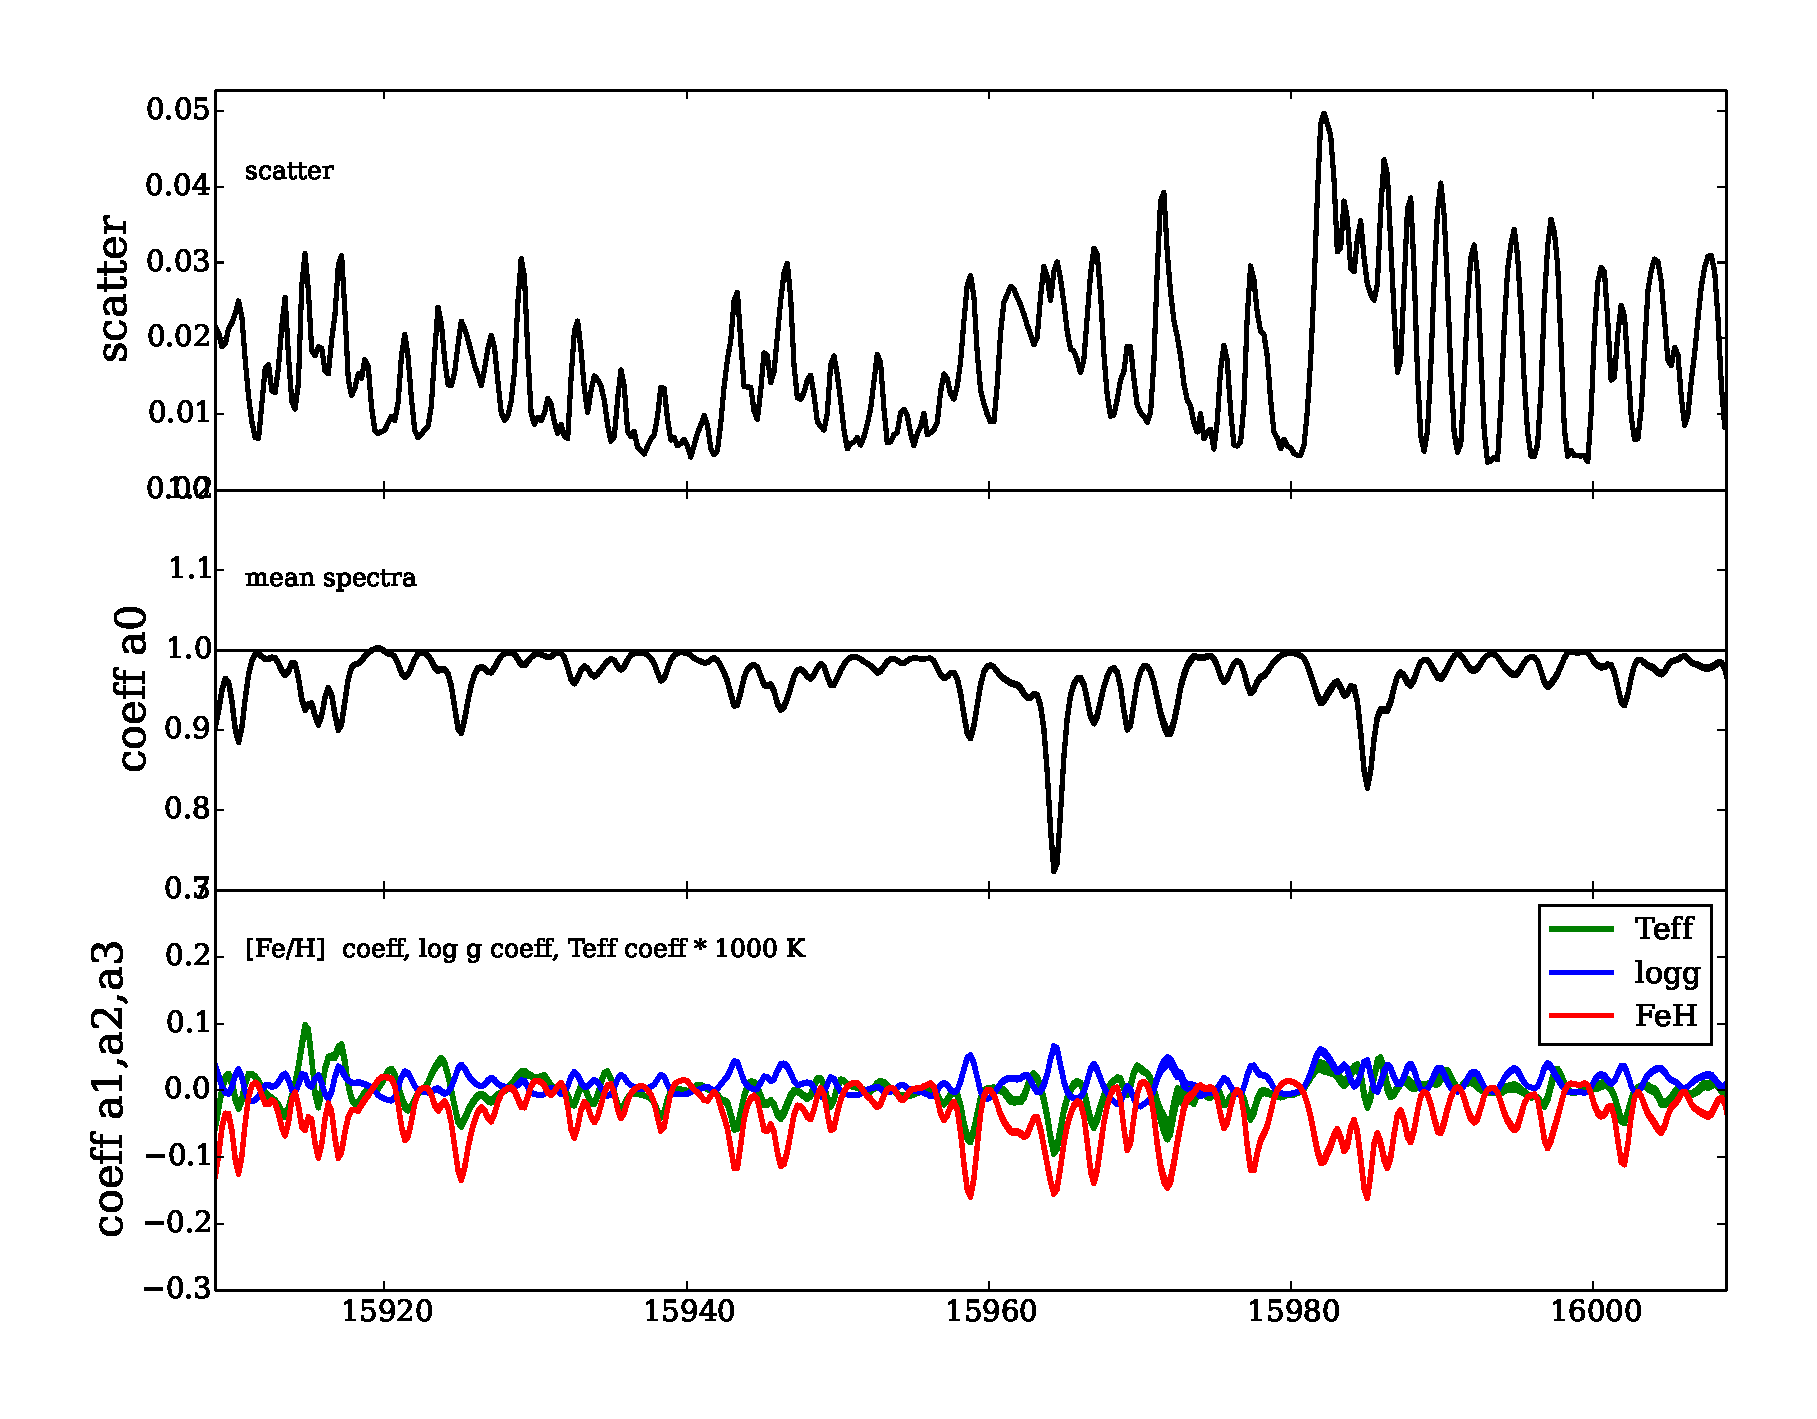
\includegraphics[width=\hsize]{./plots/R1_example.eps}
\caption{The results from the linear regression across at 100 $\AA$ sample region of spectra. The top panel shows the scatter at each wavelength, the centre panel shows the mean spectrum derived from the training set and the bottom panel shows the coefficients fit in each dimension, \teff\, \logg\, [Fe/H]. Given additional labels it will be possible to include more dimensionality, for example [$\alpha$/Fe] and [X/Fe].}
\label{fig:fits}
\end{figure}

\begin{figure}[h!]
  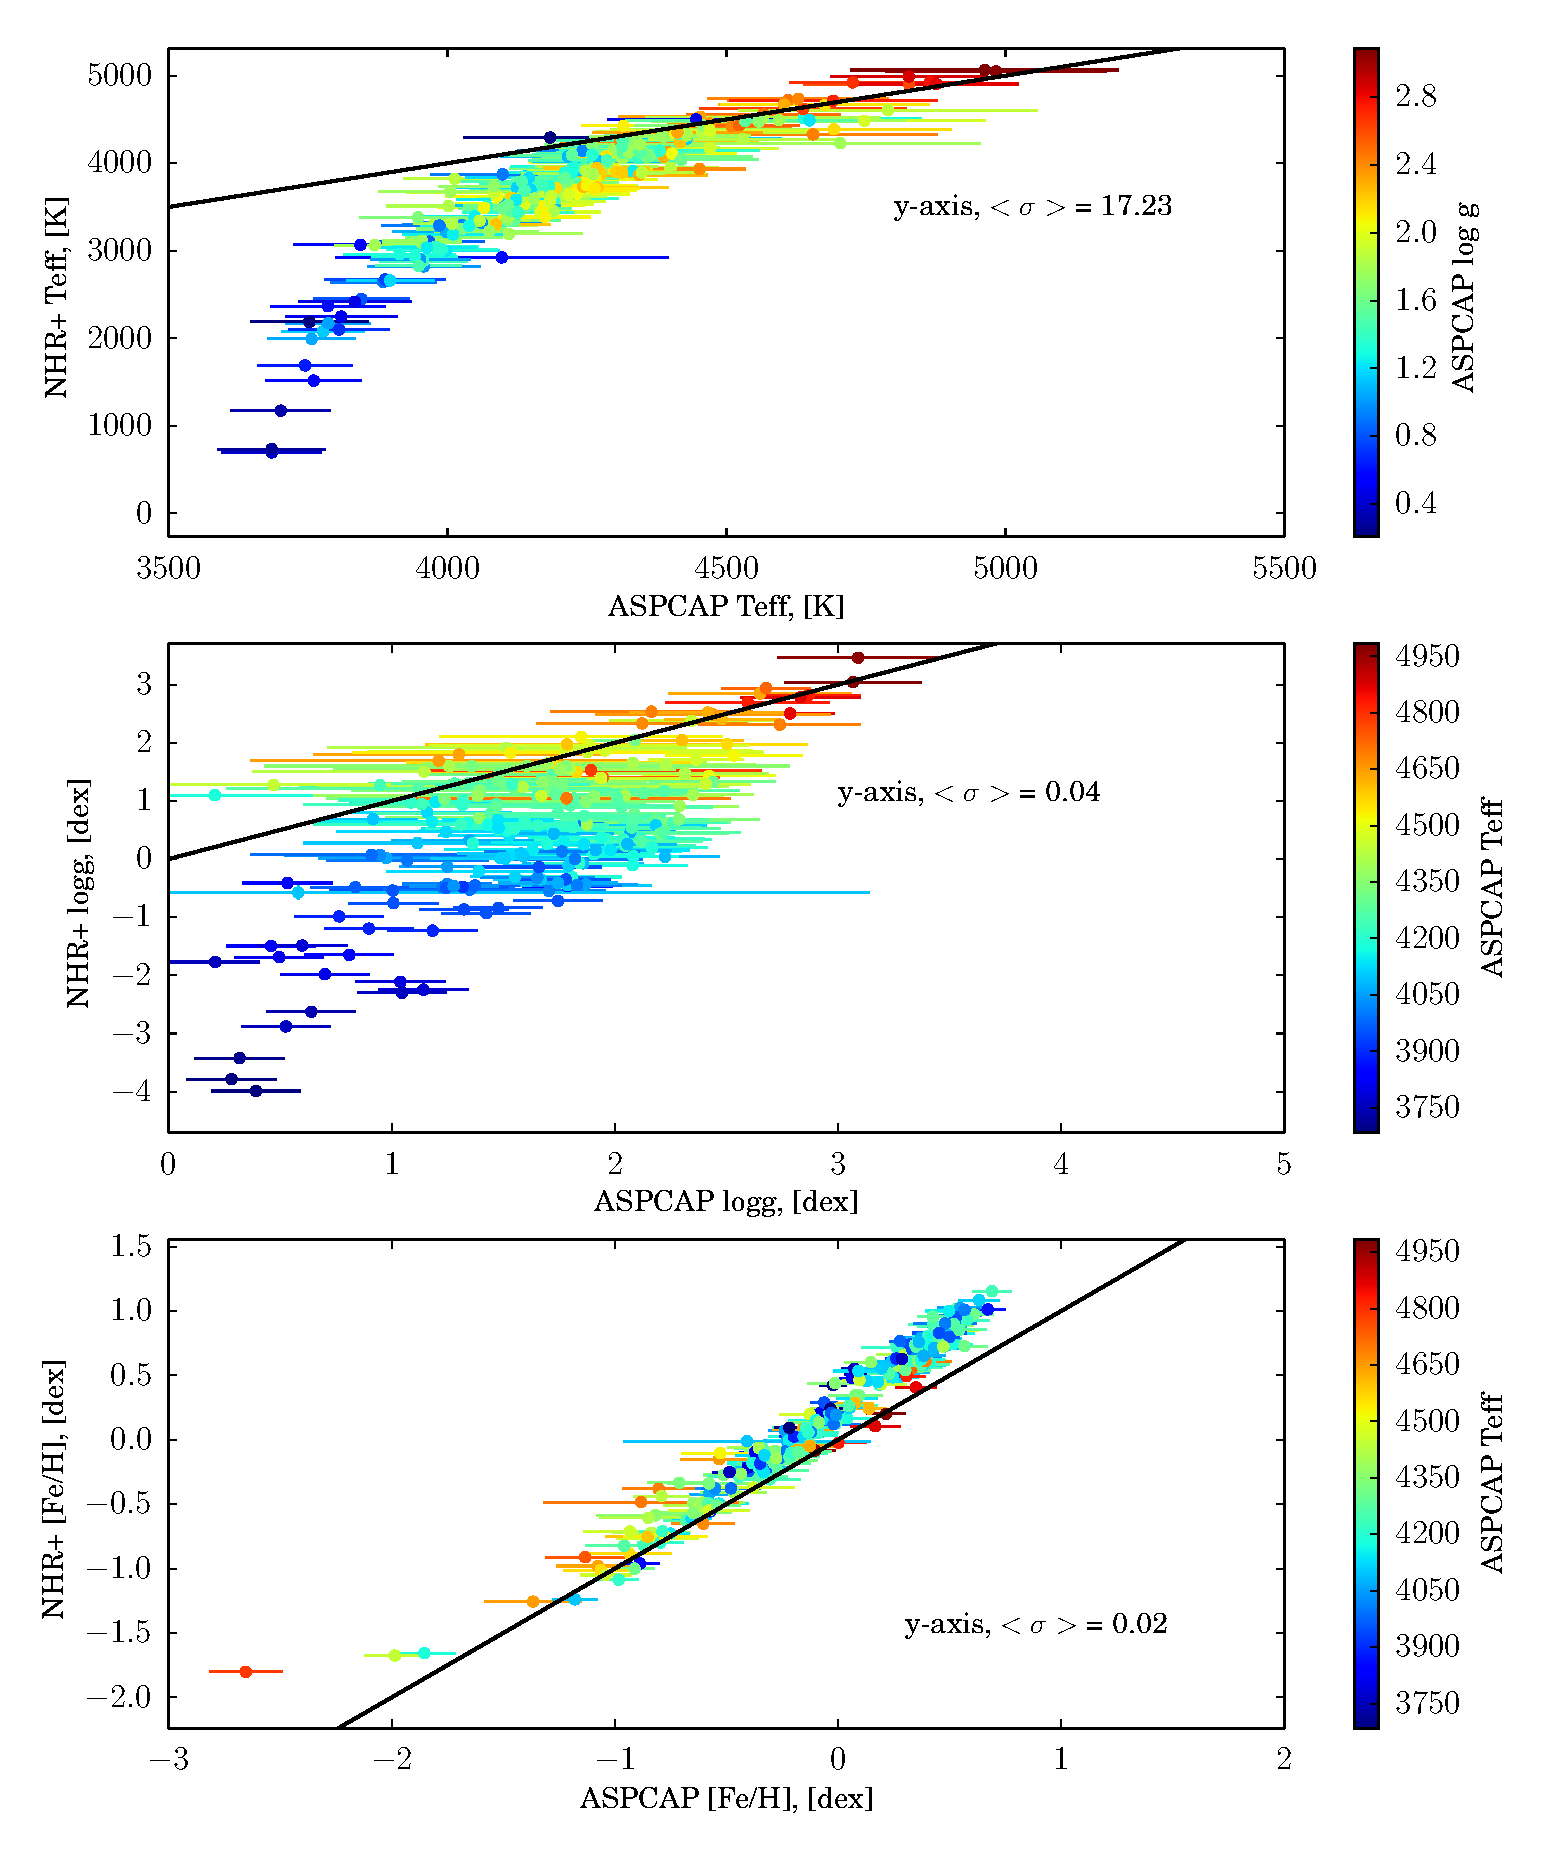
\includegraphics[width=\hsize]{./plots/fits_all3.eps}
\caption{\small{Comparison of our method with ASCAP results for the field 4332 (l,b) = (0,-5$^\circ$). The tight correlation in \teff\ and [Fe/H] suggests that these labels in the training set are very good. There is more scatter in the \logg\ panel that may not represent bad labels in the training set and therefore may not be accounted for in the non-linear model. Comparing Figure \ref{fig:index} with the bottom panel, the discontinuity at ASCAP [Fe/H] $\sim$ 0, is due to the non-linear behaviour of the [Fe/H] which is seen in the index, but which is not captured in our linear model (see Figure \ref{fig:index}).}}
\label{fig:cal}
\end{figure}

\begin{figure}[h!]
  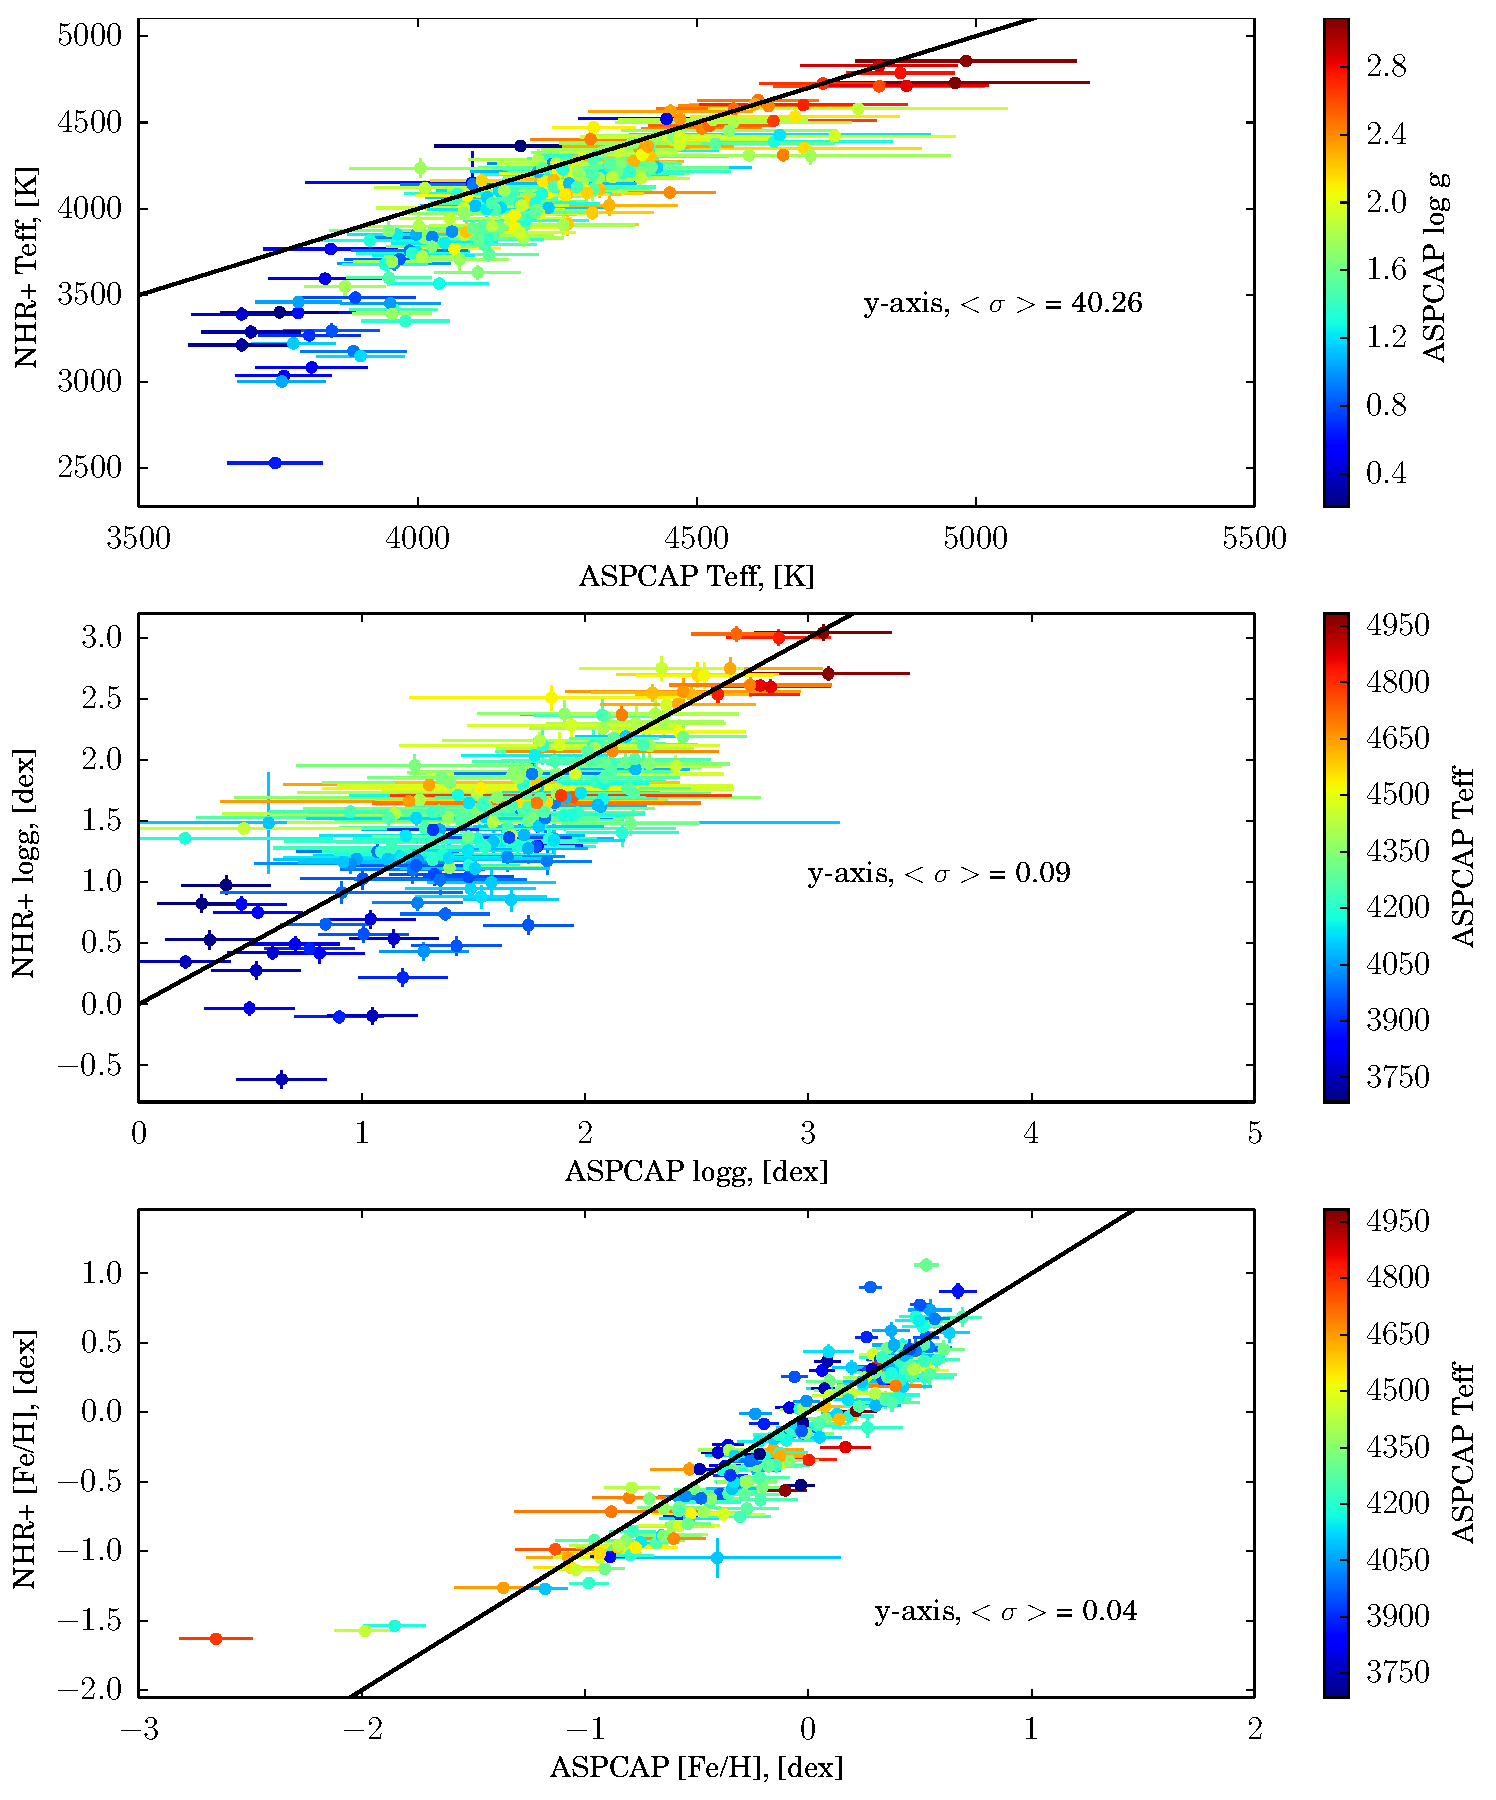
\includegraphics[width=\hsize]{./plots/fits_all3_continuumcut.eps}
\caption{\small{Comparison of our method with ASCAP results for the field 4332, using a continuum cut to select for the weak features and to exclude stronger lines. This was done to avoid the known effect of non-linearities in stronger absorption features and the cut implemented for this figure is 0.935 $<$ flux $<$ 0.99, equivalent to about 50\% of the flux of the median spectra. (note: both bounds are necessary to achieve these fits). Using weaker lines, a linear model is demonstrated to be a reasonably good model for the data. The scatter increases by about a factor of 2 in each dimension by adopting this continuum cut. }}
\label{fig:cut1}
\end{figure}

\begin{figure}[h!]
  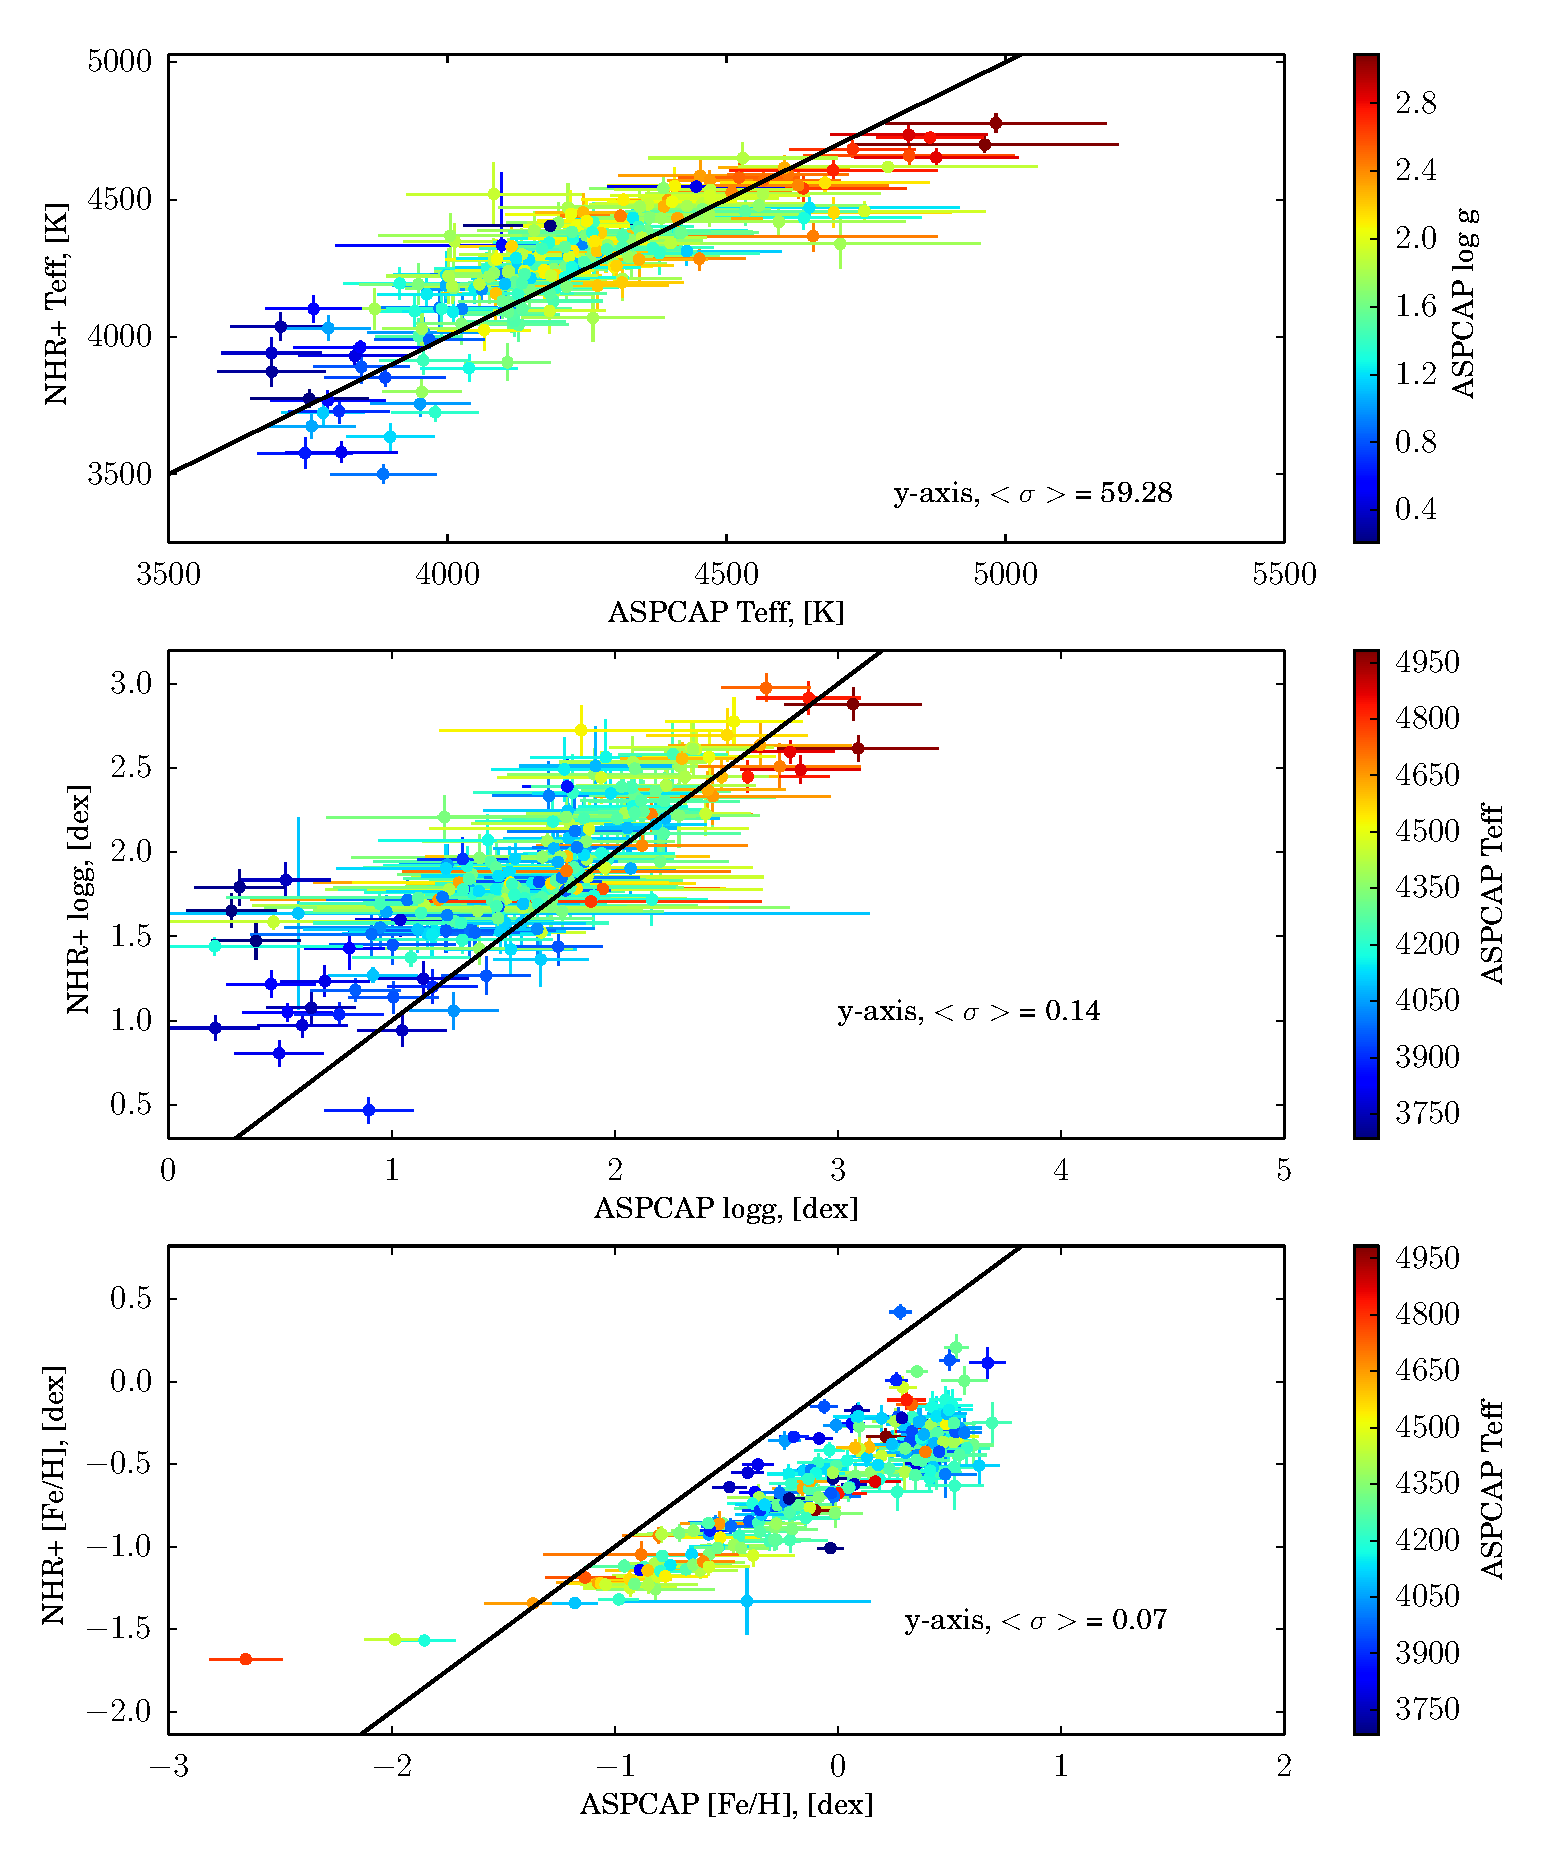
\includegraphics[width=\hsize]{./plots/fits_all3_continuumcut2.eps}
\caption{\small{As for figure \ref{fig:cut1} but using a tighter continuum cut of 0.95 $<$ flux $<$ 0.99. This demonstrates that the information for the [Fe/H] characterisation is lost at this tighter cut on the continuum, it suggests that the sensitivity of the spectra to log g is lower at the low temperature end of the spectra and the information in temperature is fairly well recovered using a linear scale for this cut in flux. } }
\label{fig:cut2}
\end{figure}

\begin{figure}[h!]
  \includegraphics[width=\hsize]{./plots/coeff_map.eps}
\caption{per pixel scaled residuals for stars ordered in [Fe/H], from the most metal poor at the bottom to the most metal rich at the top}
\label{fig:coeff}
\end{figure}

\begin{figure}[h!]
  \includegraphics[width=\hsize]{./plots/chi_map.eps}
\caption{Spectral Fingerprints for calibration clusters showing the chi2 coefficients for each star at each pixel separated into clusters from the most metal rich to the most metal poor (divided by horizontal lines) 
\textbf{To do; put clusters + [Fe/H] on other y-axis)}}
\label{fig:DNA}
\end{figure}

\begin{figure}[h!]
  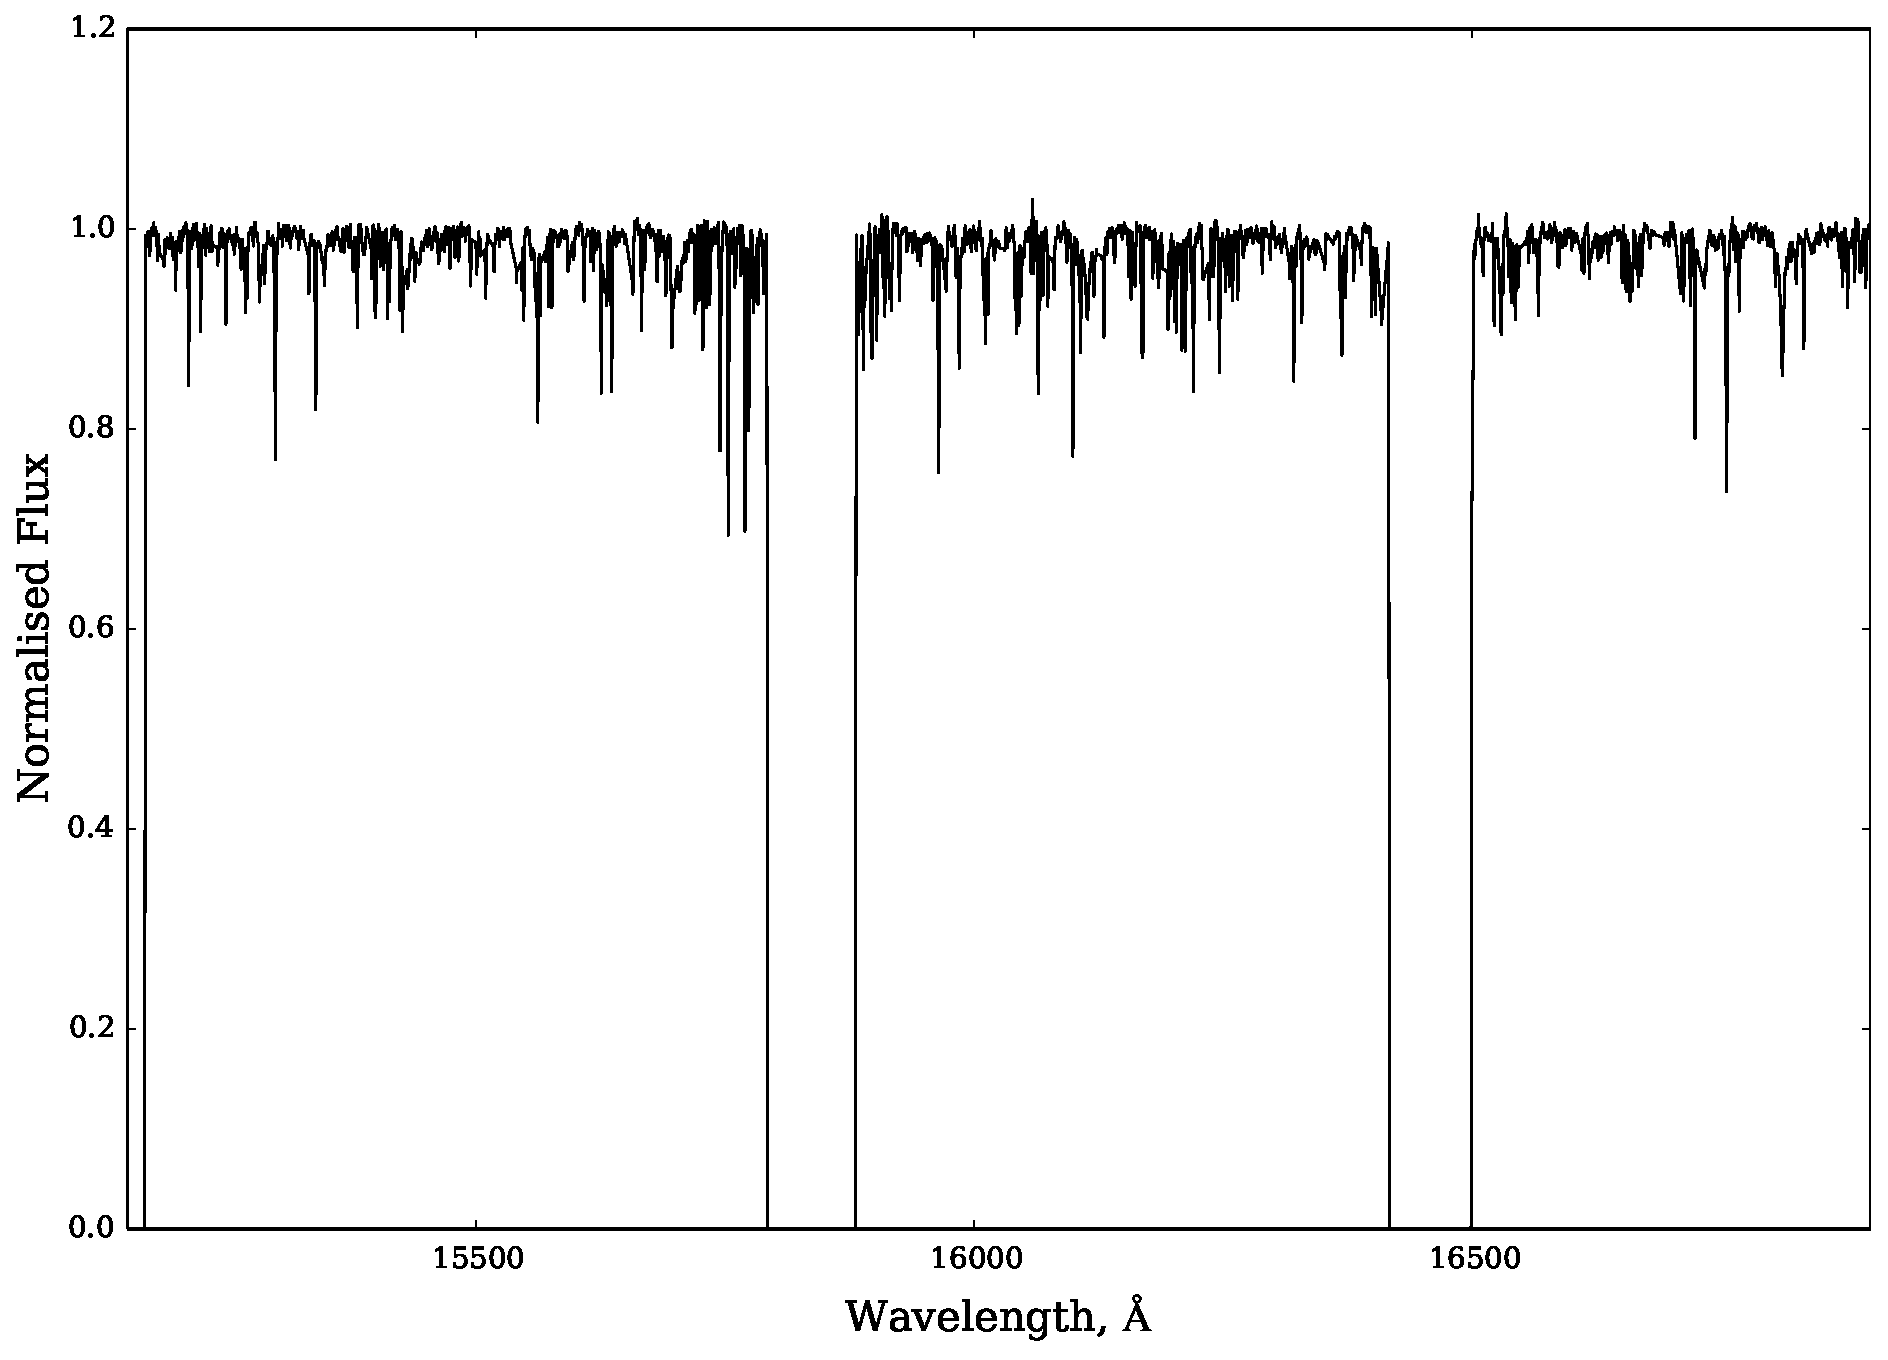
\includegraphics[width=\hsize]{./plots/normed_300.eps}
\caption{Sample continuum normalised spectra}
\label{fig:DNA}
\end{figure}

\begin{figure}[h!]
  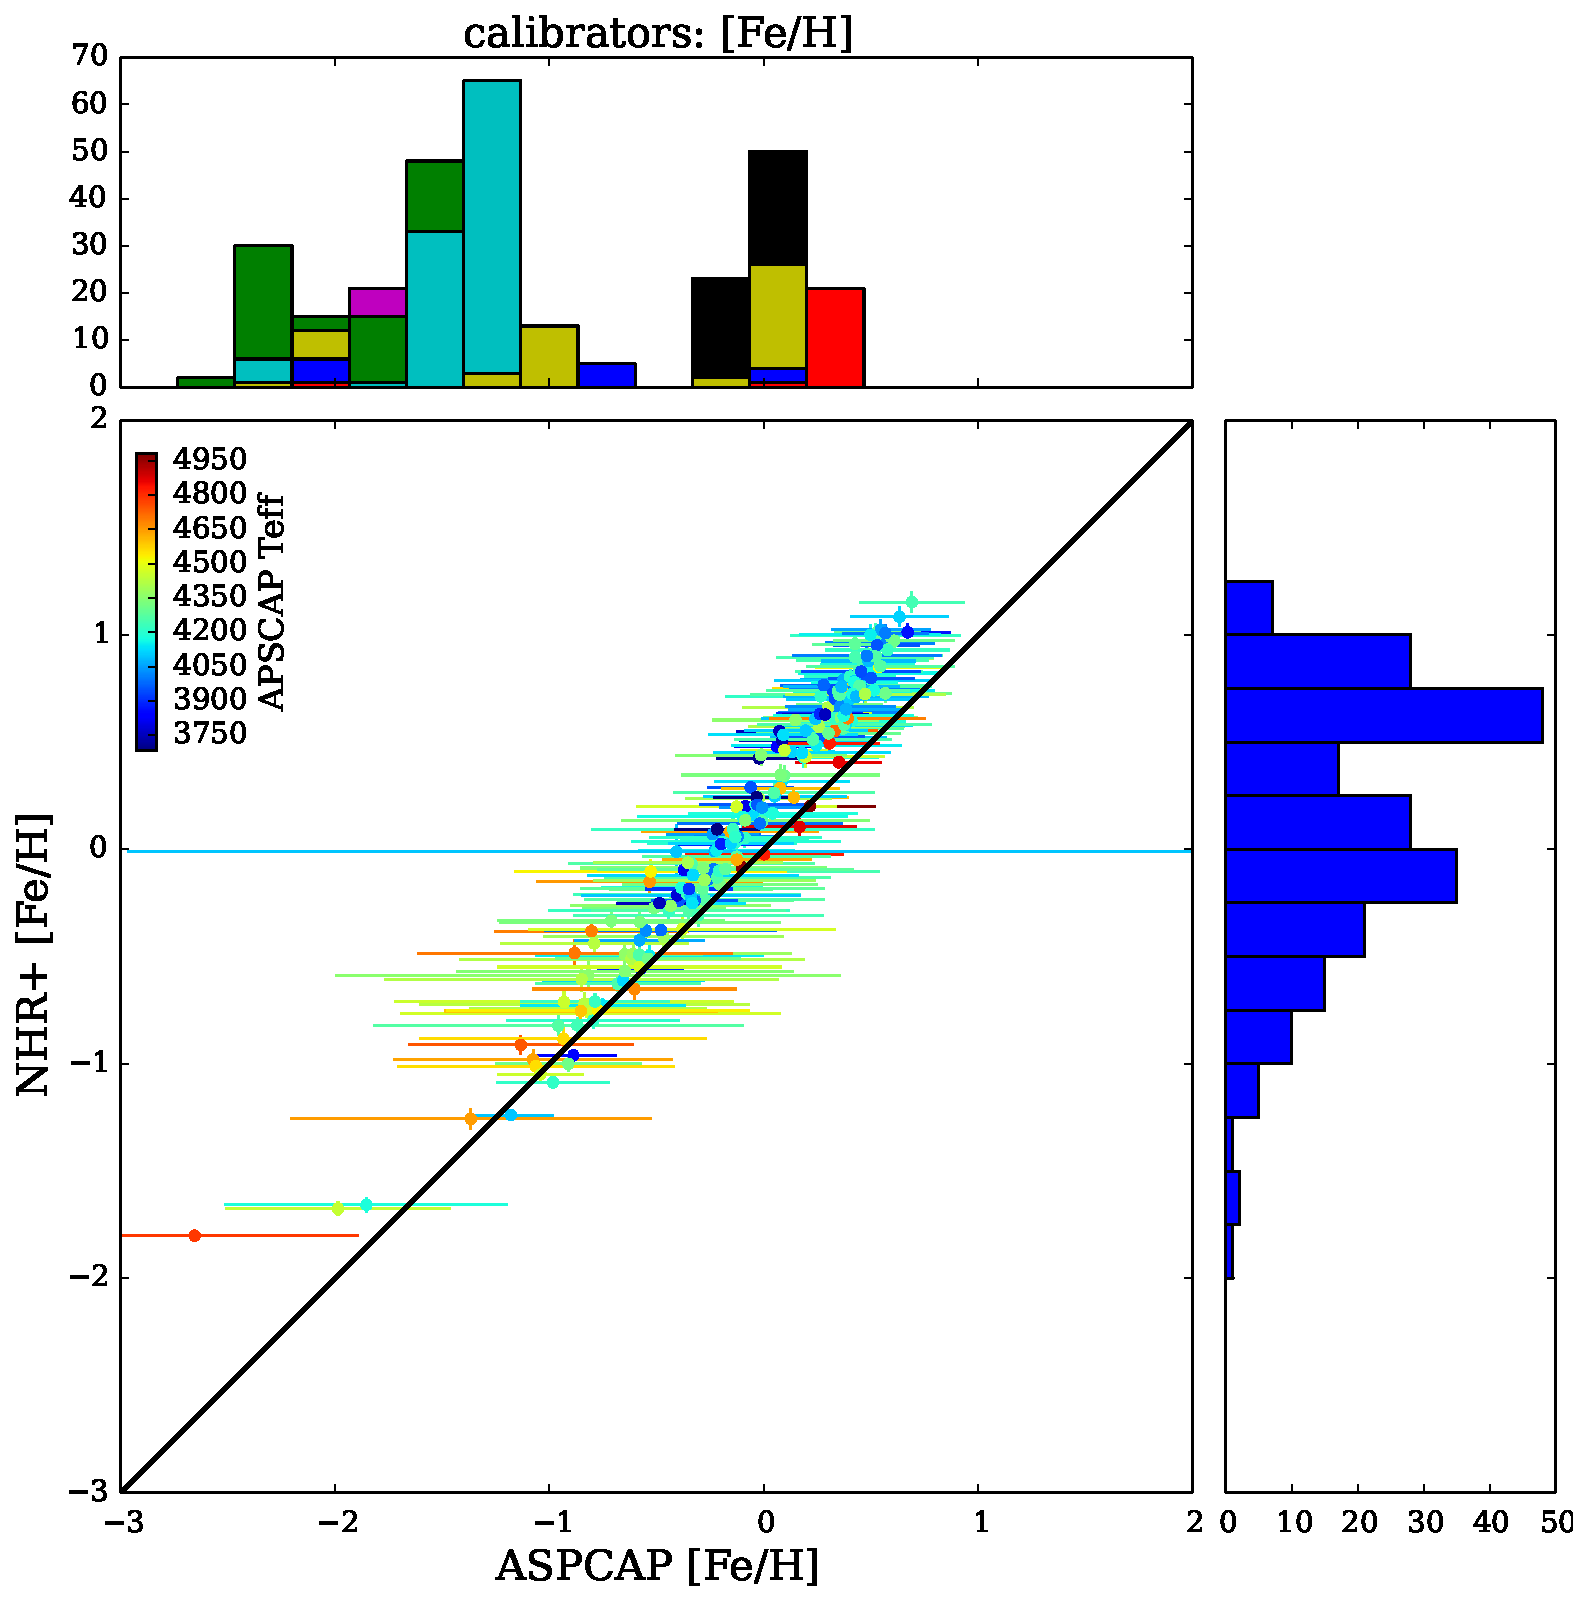
\includegraphics[width=\hsize]{./plots/cal_feh.eps}
\caption{\textbf{Need to change these to stack the histograms}: Showing the spread of calibration stars in training set across [Fe/H] - sparse sampling is not a problem in the centre for this label}
\label{fig:cal_feh}
\end{figure}

\begin{figure}[h!]
  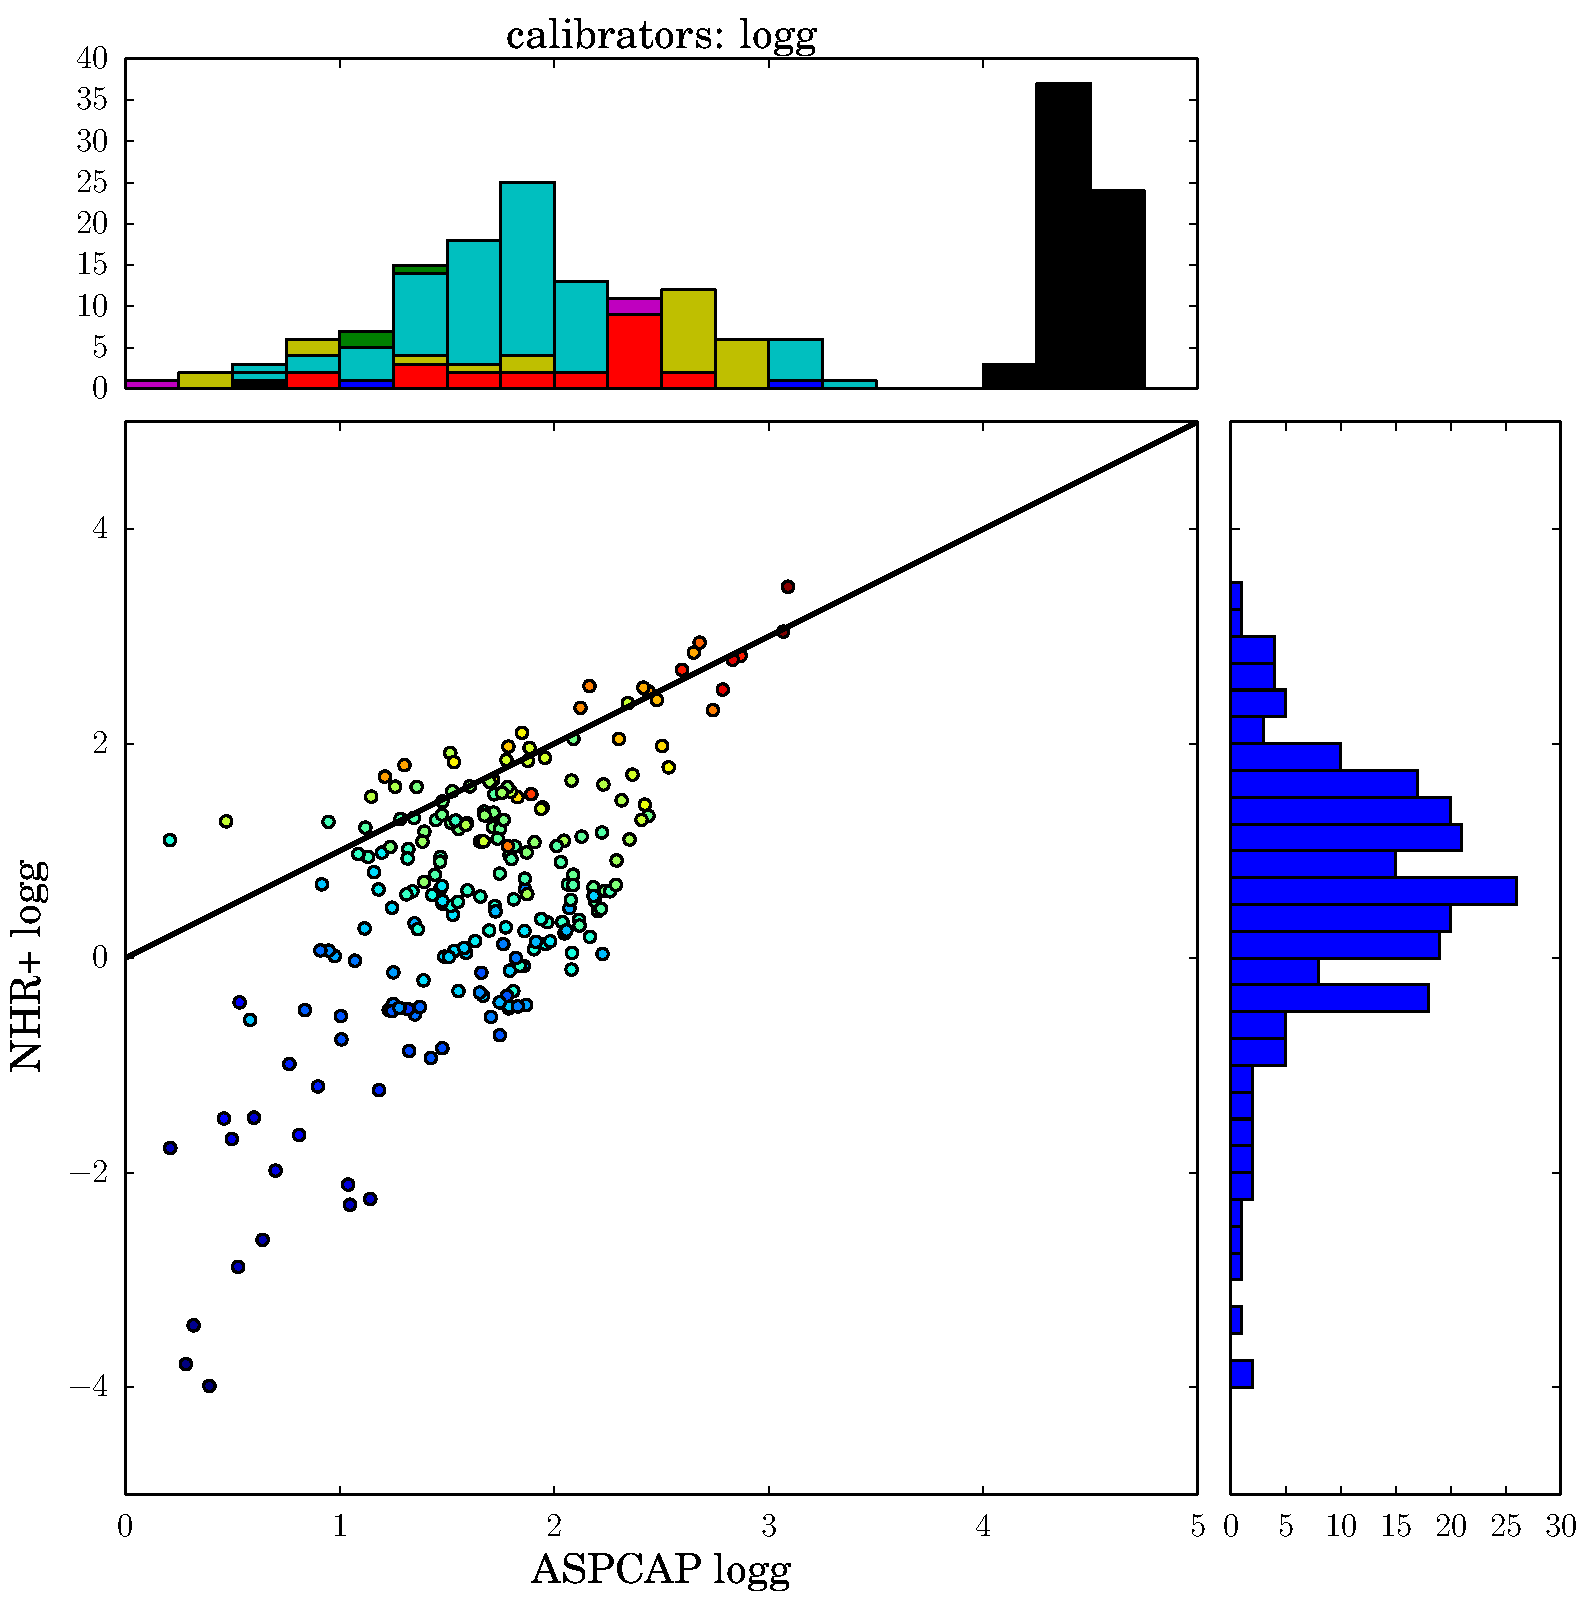
\includegraphics[width=\hsize]{./plots/cal_logg.eps}
\caption{Showing the spread of calibration stars in training set across log g ; missing sub giant stars - would be very good to have these }
\label{fig:cal_g}
\end{figure}

\begin{figure}[h!]
  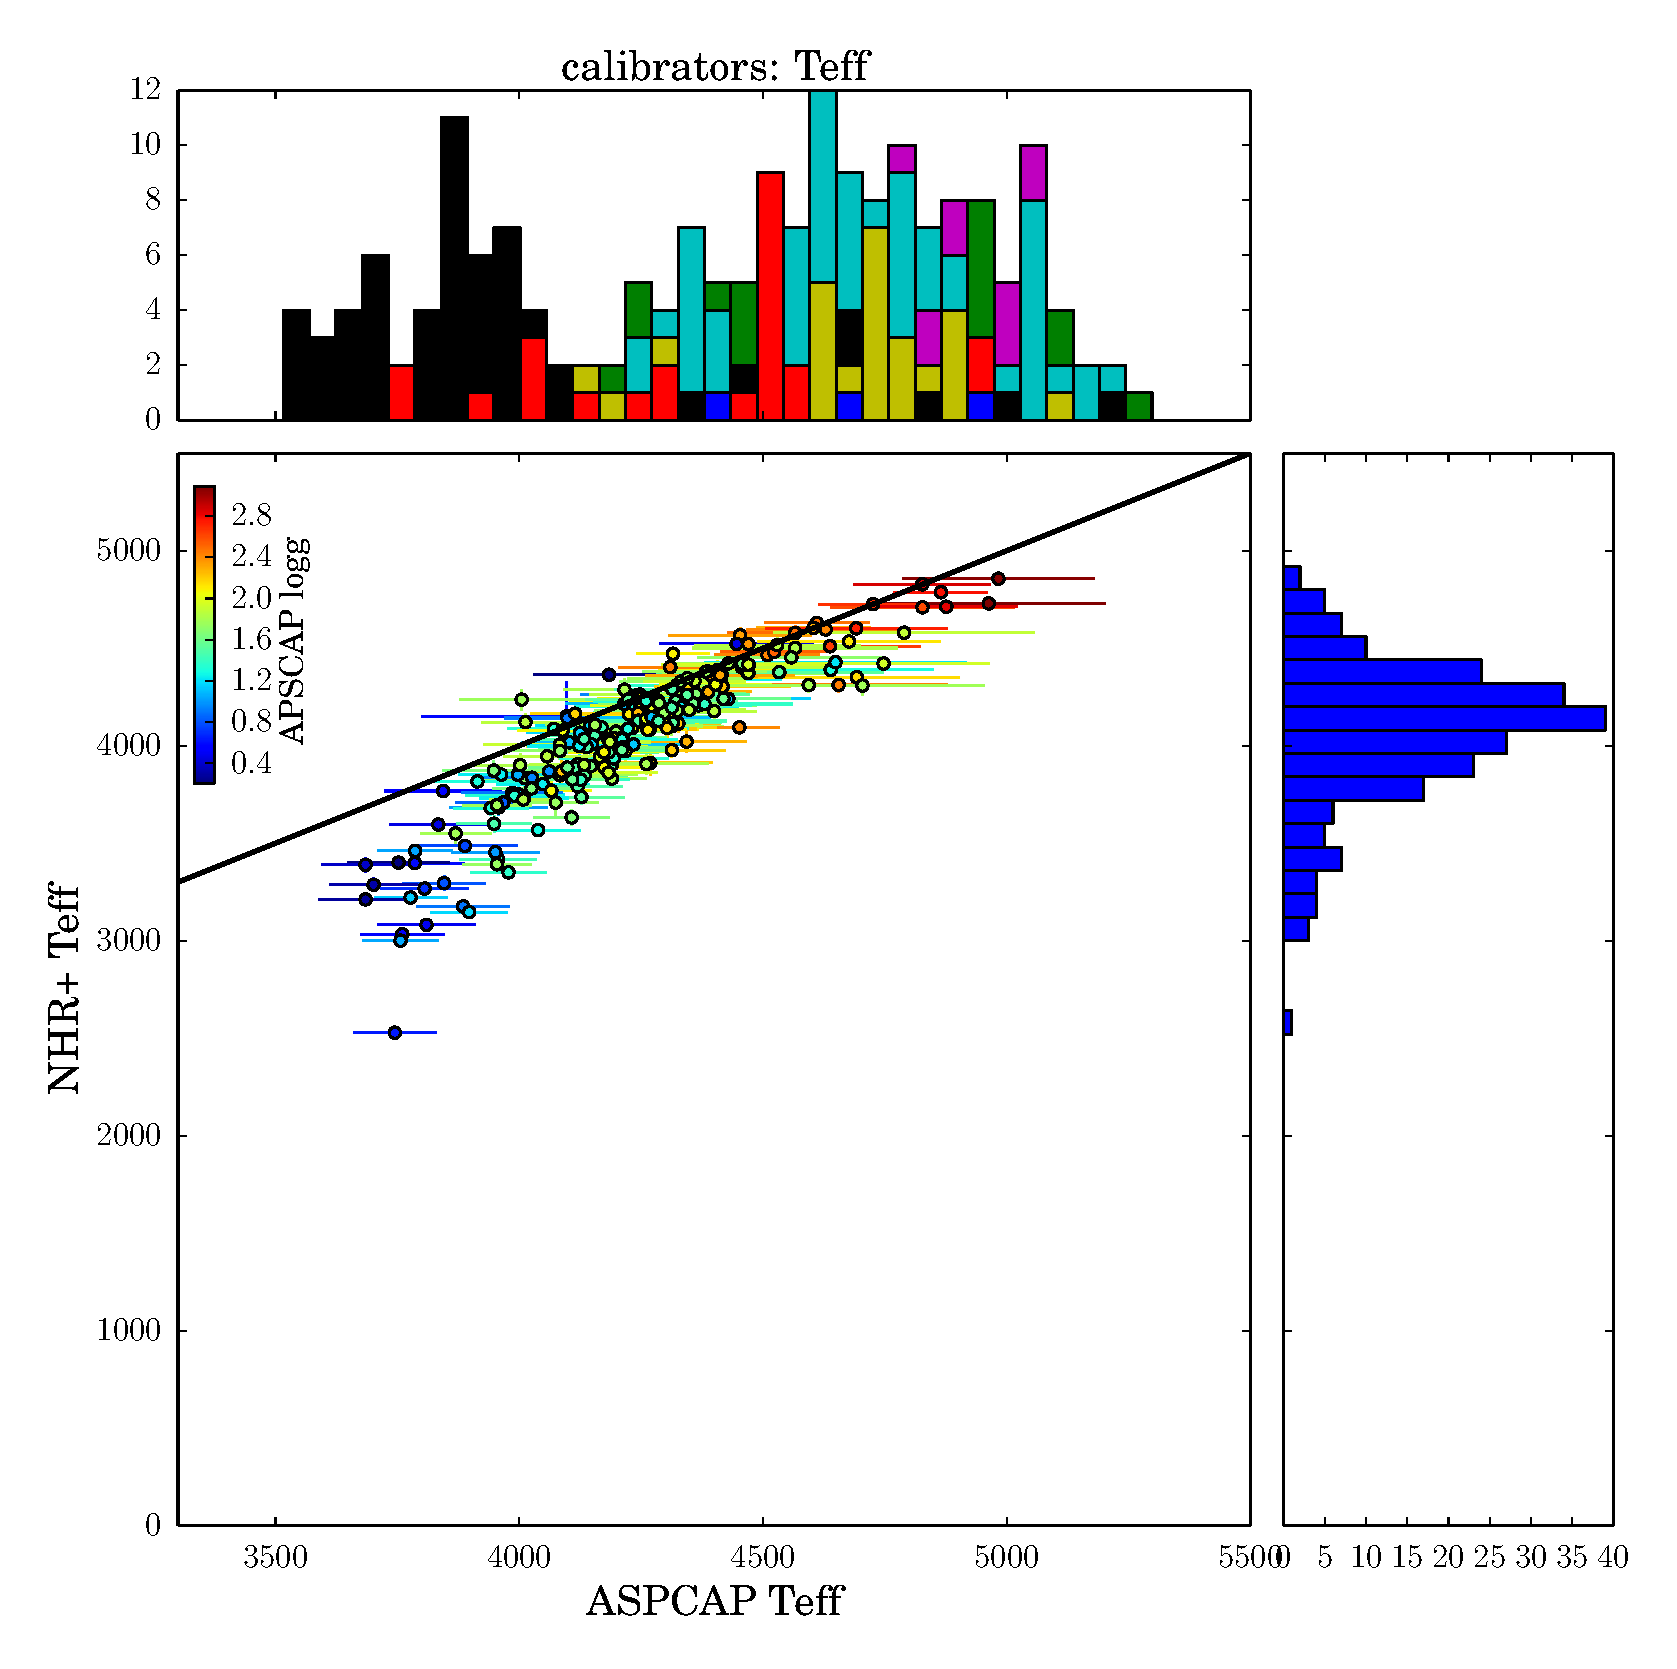
\includegraphics[width=\hsize]{./plots/cal_teff.eps}
\caption{Showing the spread of calibration stars in training set across Teff. Add error bars to these 3 figures showing the calibration.  put colourbar inside fig. have legend for the clusters as well.  }
\label{fig:cal_teff}
\end{figure}

\begin{figure}[h!]
  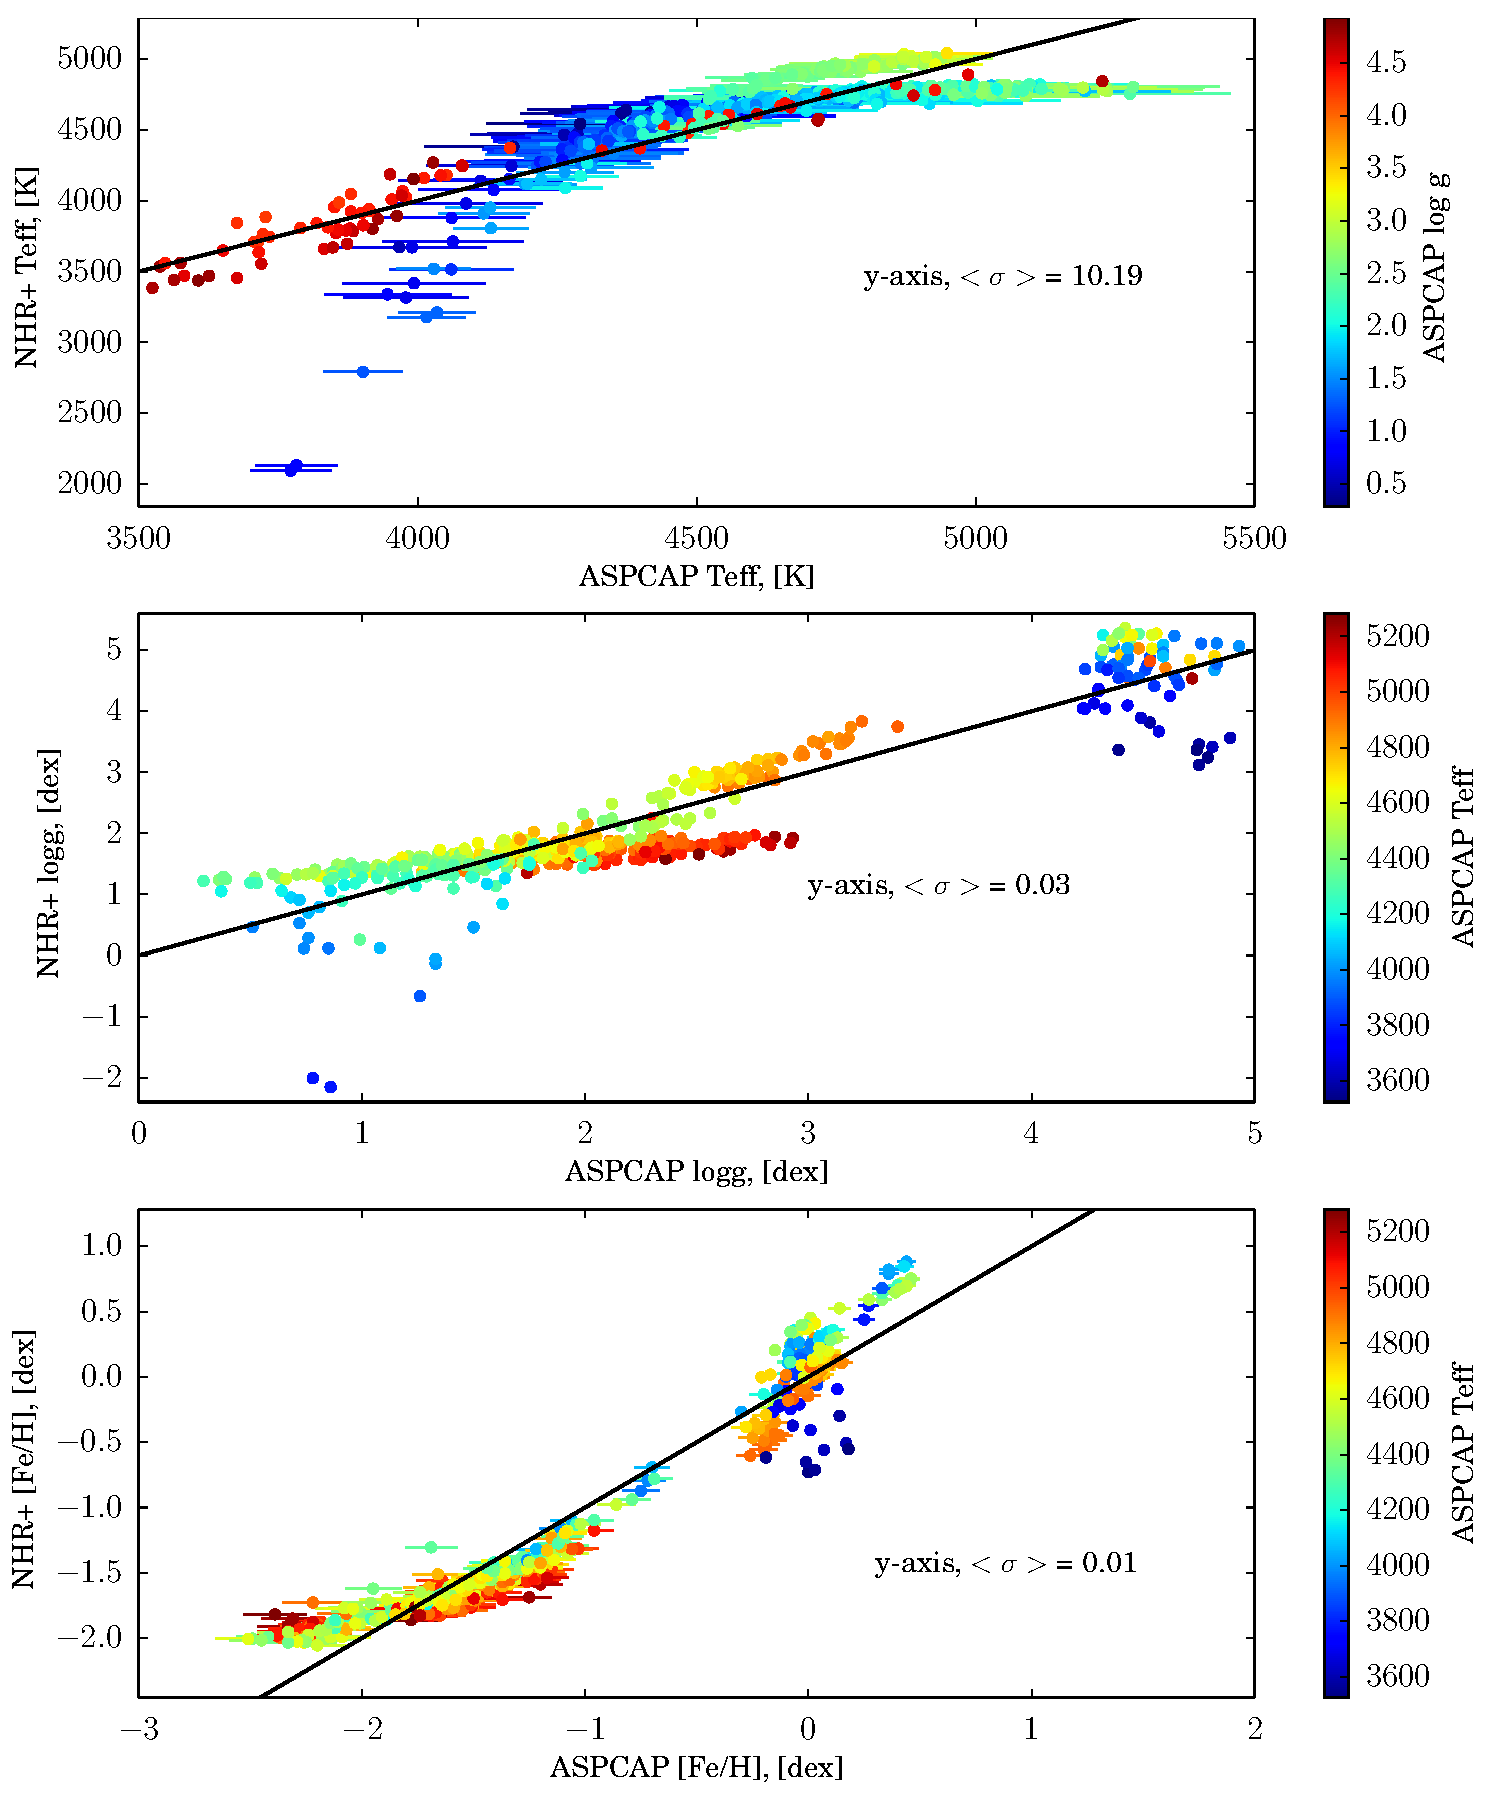
\includegraphics[width=\hsize]{./plots/fits_all3_self.eps}
\caption{this is not a cross validation this is the results of the training set run back through the code. }
\label{fig:cal_teff}
\end{figure}

\begin{figure}[h!]
  \includegraphics[width=\hsize]{./plots/linear_self.png}
\caption{this is not a cross validation this is the results of the training set run back through the code. }
\label{fig:cal_teff}
\end{figure}

\begin{figure}[h!]
  \includegraphics[width=\hsize]{./plots/nonlinear_self.png}
\caption{this is not a cross validation this is the results of the training set run back through the code. }
\label{fig:cal_teff}
\end{figure}

\begin{figure}[h!]
  \includegraphics[width=\hsize]{./plots/4332_all.png}
\caption{this is not a cross validation this is the results of the training set run back through the code. }
\label{fig:cal_teff}
\end{figure}

\begin{figure}[h!]
  \includegraphics[width=\hsize]{./plots/Field_4332_nonlinear.png}
\caption{this is not a cross validation this is the results of the training set run back through the code. }
\label{fig:cal_teff}
\end{figure}






\end{document}

%abstract notes%



%
%
%
%
%, using label-transfer from stars with defined labels (e.g. of \teff, \logg, \feh).
%
%Using the APOGEE dataset and a training set of globular and open clusters observed by APOGEE, we demonstrate that this approach is simple, fast and extremely successful in deriving stellar parameters for APOGEE data. As we exploit every pixel in the spectra, the intrinsic errors in the method are small, which facilitates going to much lower SNR than current approaches. $< $quantify this$>$. As part of this proof of concept we include a catalogue of \teff\, \logg\ and [Fe/H] for 60K stars observed in APOGEE for DR10, including parameters for dwarf as well as giants, which have not been previously reported. \\

%This method is directly transferable between surveys and wavelength regions and relies on a training set of spectra with well defined labels. These labels may include stellar parameters of \teff\, \logg\ and [Fe/H], [$\alpha$/Fe] and individual abundances [X/Fe]. Via this method we characterise how every pixel in a spectra contributes to defining the labels of a star and in doing this, we utilise all of the information within the stellar spectra. \\

%We present a method which enables a wavelength and model independent determination of stellar parameters using label-transfer from a training set of real data with known labels. This approach does not require an intricate line-list characterisation in each new wavelength region observed and makes stellar parameter determination accessible to the community. This technique exploits all of the information in the stellar spectrum and it is therefore possible to determine stellar parameters within at a significantly lower signal to noise than minimisation techniques, for a given uncertainty on the labels. \\

%We present a method to estimate stellar parameters and abundances (or "labels") for APOGEE spectra that does not require direct comparison to synthetic model spectra. Our method, called \tc, transfers labels (\teff, \logg and [Fe/H]) from a training set of data whose parameters are well determined (i.e. members of open and globular clusters) to the entire set of stars in the survey. We show we can reproduce the stellar parameters for the APOGEE survey for DR10 and achieve this at a fraction (25\%) of the signal to noise required by minimisation techniques. We obtain this performance via characterising the relationship between the labels of the stars in our training set and their flux, at each pixel. Our method is expandable to additional labels and relevant for chemical tagging. This approach argues for an established set of standard stars with well-determined labels. Given such standard calibrators, it is possible, via this technique of label-transfer, to place every stellar survey of the Milky Way on the same stellar parameter scale and homogeneously map the stellar population of the Milky Way from Northern and Southern hemispheres and using different wavelength regions.


%This method has has important applications for homogenising all large surveys and chemical tagging, for which this approach is ideal.

enables the homogenisation of northern and southern observing programmes across different wavelength regions given adopted standard calibrator stars. 


- allows information in entire region of  a spectrum to be captured and understood. 


%Stellar models are not yet complete and accurate/linelists are not yet complete and accurate/each new survey has own independent implementation of stellar parameter and abundance determination with a lot of repeated effort/multiple surveys on different scales/methods required for chemical tagging.\\
%Established standard stars with labels including in [X/Fe], which can be re-observed as part of every new large survey and serve as the training set for the method, has important applications for homogenising all large surveys and chemical tagging, for which this approach is ideal. \\
%


INTRODUCTION
###


%Our pursuit of understanding flux with respect to stellar labels has achieved a number of outcomes. 
%1) We present a methodology to use label-transfer to efficiently and effectively determine stellar parameters for a large survey, using the example of the APOGEE survey 2) We demonstrate that by adopting a mathematical approach the signal to noise required for at least nominal stellar parameters is lower than by aiming for a minimisation driven determination 3) We are able to show, which we do visually, the fingerprints of our stellar spectrum for each label - we can graphically and quantatively describe how at each pixel, the flux varies with the label 4) We propose this technique as relevant for chemical tagging. We will add more labels including alpha, X/Fe and age - same idea just more labels. 

%We started with most simple - linear, found quadratic and go to fully bayes. gaussian process+ at other end of this. 

XX I need to put in a figure here of the quadratic case for the fits showing how the flux changes with labels but NORMALISE THIS - currently not done relatively to each other - need to see relative scale XXX. 

%Key - relies on training set and how good this is. 
%We seek not to find a best fit model.
%continue to be updated and improved, as well as adopted calibration scales and techniques. 
%and the outputs of which are sensitive to ab-initio assumptions, post calibrations and offset from scales of other surveys. 
%Furthermore, this implementation makes stellar parameter determination itself accessible to the wider community. \\

%There are now numerous large stellar surveys of the Milky Way, each of which is independently working to determine stellar parameters across different wavelength regions. Our aim is to provide a generalised tool - decentralised parameter determination, that can in principle put everything on the same scale. Demonstrated limitations of this example - missing calibrators across some of the range, e..g teff.

%Challenges of stellar parameter estimation.

%In principle there could be data-driven models.

%Data-driven models would permit ``label-transfer''.
%This is especially important if we want optical models to provide labels for infrared surveys (and so on).

%APOGEE provides a great data set for exploring these issues. Large homogenous datasets make this possible for the first time. 

%Also avoids issue of stellar models once have well characterised set, given any wavelength for calibration and is very fast + generalised. 
%issues - cite Meszaros paper for typical implementation. 

We implement this technique as a method to systematically and optimally exploit the information in stellar spectra within large homogeneous datasets.  Our method avoids explicit stellar models and the data itself is the basis of the characterisation. Models are required ab initio and can be implemented at an independent wavelength range, to set the labels for the calibration data.  We apply the primary spectral labels of \teff\, \logg\, [Fe/H] and this process can be extended and applied in N dimensions given well labeled training sets. Calibration sets, of open and globular cluster data, are critical to enable this method which can in principle be implemented with synthetic libraries but this folds in unphysical residuals. We present a general method by using the APOGEE example, characterising the APOGEE spectra and demonstrating how dimensionality of the calibration set can be applied to interpret APOGEE data. 

Motivated by the idea of fingerprinting spectra in the spirt of chemical tagging and developing robust methods that allow the spectra to be mapped in full as a function of its labels. Reverse philosophy to a lot of current techniques were individual lines are the focus, here we disregard what they are and examine impartially. This may reveal information that may not be obvious or otherwise determined. note - Can I find an example of this for the paper? 

%map labels of test set onto the larger set of data
###

OLD SPECTRAL MODEL BELOW

\section{Spectral model}

The model is that the observed, continuum-normalized spectrum, at each
wavelength, can be explained as a linear combination of real-valued
``labels'', or a linear combination of functions of those labels.
Here the labels will be things like effective temperature $\teff$,
logarithmic surface gravity $\logg$, and metallicity $\feh$.
Additionally, the model is that at each wavelength, the observed
spectrum will deviate from the linear combination by some additive
noise contribution, some of which comes from photon noise and
sky-subtraction noise and other instrumental contributions, and some
of which is an intrinsic scatter, presumed independent at each
wavelength.
The model is built using ``training data'' (with known labels) and then
used to tag (or infer labels for) the ``test data''.

In the training data there will be $N$ spectra $n$, each of which has
a continuum-normalized flux measurement $y_{n\lambda}$ at wavelength
$\lambda_\lambda$, and an associated uncertainty variance
$\sigma_{n\lambda}^2$ from finite photon counts and instrumental effects.
If there are missing flux values in the training data, these can be
handled by setting variances to something very large (or inverse
variances to something very small).
Each of the training spectra $n$ has $K$ labels $x_{nk}$, each of which
is (for now) presumed to have negligible uncertainty.
The general model is
\begin{eqnarray}
y_{n\lambda} &=&
 Y(\set{x}_n\given\set{\theta}_\lambda) + [s_\lambda^2 + \sigma_{n\lambda}^2]^{1/2}\,\xi_{n\lambda}
\label{eq:model}\\
\set{x}_n &\equiv& [x_{n1}, x_{n2}, \cdots, x_{nK}]
\quad,
\end{eqnarray}
where $Y()$ is some (possibly complicated) function of the full set
of $K$ labels, $\set{x}_n$ is a vector or blob of the $K$ labels for spectrum $n$,
$\set{\theta}_\lambda$ is the set of parameters controlling the
function $Y()$ at wavelength $\lambda_\lambda$, $s_\lambda^2$ is an
intrinsic variance for the model at wavelength $\lambda_\lambda$, and
$\xi_{n\lambda}$ is a Gaussian random number with zero mean and unit
variance.
That is, we have assumed that the noise is Gaussian, zero mean, and
independent for every measurement.
This model leads to the single-pixel log-likelihood function
\begin{eqnarray}
\ln p(y_{n\lambda}\given\set{\theta}_\lambda,s_\lambda^2) &=&
 -\frac{1}{2}\frac{[y_{n\lambda} - Y(\set{x}_n\given\set{\theta}_\lambda)]^2}{s_\lambda^2 + \sigma_{n\lambda}^2}
 -\frac{1}{2}\ln(s_\lambda^2 + \sigma_{n\lambda}^2)
 -\frac{1}{2}\ln 2\pi
\label{eq:like1}\\
\set{x}_n &\equiv& [x_{n1}, x_{n2}, \cdots, x_{nK}]
\quad.
\end{eqnarray}
Since all the spectra and pixels are treated as independent, each
wavelength $\lambda_\lambda$ can have its parameters
$[\set{\theta}_\lambda,s_\lambda^2]$ inferred independently, and all the
individual-spectra log-likelihoods can be added together to make
\begin{eqnarray}
\ln p(\set{y}_\lambda\given\set{\theta}_\lambda,s_\lambda^2) &=&
 \sum_{n=1}^N \ln p(y_{n\lambda}\given\set{\theta}_\lambda,s_\lambda^2)
\label{eq:like}\\
\set{y}_\lambda &\equiv& [y_{1\lambda}, y_{2\lambda}, \cdots, y_{N\lambda}]
\quad,
\end{eqnarray}
where $\set{y}_\lambda$ is the vector of spectral flux values for
the $N$ objects all at wavelength $\lambda_\lambda$.
We can set the parameters $[\set{\theta}_\lambda,s_\lambda^2]$ either by
optimizing the likelihood (\ref{eq:like}) or by applying priors and
performing some kind of probabilistic inference (with, say, Markov
Chain Monte Carlo techniques).
Here we will optimize for now.

In this \sectionname, we are treating the function parameters
$\set{\theta}_\lambda$ and the scatter $s_\lambda^2$ as free parameters, and the
labels $x_{nk}$ as fixed.
The likelihood function (\ref{eq:like}) is presented as being a
function of these free parameters.
In the next \sectionname, the tables will turn, and we will treat the
function parameters $\set{\theta}_\lambda$ and scatter $s_\lambda^2$ as fixed and
the labels $x_{nk}$ as parameters.
The difference is that here we are treating the training data as
having perfectly known labels, and later we will be inferring labels for
new spectra.

The simplest spectral model is that in which the functions $Y()$ are
linear in the labels:
\begin{eqnarray}
Y(\set{x}_n\given\set{\theta}_\lambda) &=&
 a_{\lambda 0} + \sum_{k=1}^K a_{\lambda k}\,[x_{nk} - \mean{x_k}]
\label{eq:linear}\\
\set{x}_n &\equiv& [x_{n1}, x_{n2}, \cdots, x_{nK}]
\\
\set{\theta}_\lambda &\equiv& [a_{\lambda 0}, a_{\lambda 1}, \cdots, a_{\lambda K}]
\quad ,
\end{eqnarray}
where the $a_{\lambda k}$ are linear coefficients, and
the $\mean{x_k}$ are offsets (possibly means of the training data) to
keep the model ``pivoting'' around a reasonable point in tag space.
This linear-in-labels form (\ref{eq:linear}) has many useful and
excellent properties.
The first is that optimization of the model, at fixed scatter
$s_\lambda^2$ is a pure linear-algebra operation (weighted least
squares); simultaneous optimization of all the parameters
$[\set{\theta}_\lambda,s_\lambda^2]$ is only nonlinear in the $s_\lambda^2$
parameter.
The second is that the tag inference (label-transfer; described in the
next Section) on the test data will have a very simple form.
The third is that the coefficients $a_{\lambda 0}$, seen as a discrete
function of wavelength $\lambda_\lambda$, can be seen as an estimate of
the \emph{mean spectrum} (provided that the offsets $\mean{x_k}$ are
the mean tag values over the $N$ training spectra); and the
coefficients $a_{\lambda k}$ can be seen as the mean first derivatives of
the expected spectrum with respect to each of the $k$ labels, estimated
over the range of the training data.

The results for the linear-in-labels model (\ref{eq:linear}) are shown
in Figures~XXX through YYY.  They show... departures from
linearity... outliers...

...what are we doing about outliers?  If anything?  Perhaps in discussion too...

- discuss how this method can be improved using priors as have this information e.g know space in Teff-logg that stars should lie in. 

...Of course weak lines might be closer to linear... what happens when
we restrict to weak lines?..

...is this a good model?  No; how do we know?

The (perhaps) second-simplest spectral model is that in which the
functions $Y()$ are quadratic in the labels:
\begin{eqnarray}
Y(\set{x}_n\given\set{\theta}_\lambda) &=&
 a_{\lambda 0} + \sum_{k=1}^K a_{\lambda k}\,[x_{nk} - \mean{x_k}]
 + \sum_{k=1}^K \sum_{k'=k}^K a_{\lambda kk'}\,[x_{nk} - \mean{x_k}]\,[x_{nk'} - \mean{x_{k'}}]
\label{eq:quadratic}\\
\set{x}_n &\equiv& [x_{n1}, x_{n2}, \cdots, x_{nK}]
\\
\set{\theta}_\lambda &\equiv& [a_{\lambda 0}, a_{\lambda 1}, \cdots, a_{\lambda K},
                            a_{\lambda 11}, a_{\lambda 12}, \cdots, a_{\lambda KK}]
\quad ,
\end{eqnarray}
where the $a_{\lambda k}$ and $a_{\lambda kk'}$ are linear coefficients, and
the $\mean{x_k}$ are offsets (possibly means of the training data) to
keep the model ``pivoting'' around a reasonable point in tag space.
This quadratic-in-labels form (\ref{eq:quadratic}) is similar to and
different from the linear-in-labels form (\ref{eq:linear}) in a number
of ways.
It is still the case that optimization of the model, at fixed scatter
$s_\lambda^2$ is a pure linear-algebra operation (weighted least
squares).
However, tag inference (described in the next Section) on the test
data will no longer be simple; it will now require non-linear
optimization.
The coefficients $a_{\lambda 0}$ can still be seen as an estimate of the
\emph{mean spectrum} (provided that the offsets $\mean{x_k}$ are the
mean tag values); the first-order coefficients $a_{\lambda k}$ can still
be seen as first derivatives of the expected spectrum with respect to
each of the $k$ labels, but now evaluated at the mean spectrum; the
second-order coefficients $a_{\lambda kk'}$ can now be seen as mean
second derivatives of the expected spectrum with respect to pairs of
labels $k$ and $k'$.

The results for the quadratic-in-labels model (\ref{eq:linear}) are shown
in Figures~XXX through YYY.  They show... departures from
linearity... outliers... is it really a better model?..

\section{Parameter estimation}

In the previous \sectionname, we built data-driven spectral models
from training data.
These models have the property that, given labels, they can be used to
predict continuum-normalized flux, up to observational and intrinsic
scatter.
In this \sectionname, we are going to solve the inverse problem; we
are going to presume that we have spectra, but we don't have labels.
In this case, we will use inference to obtain labels for the untagged
spectra.
These untagged spectra will be referred to as the ``test data'' in
what follows.

In the test data there will be $M$ spectra $m$, each of which---as in
the training data---has a continuum-normalized flux measurement
$y_{m\lambda}$ at each of $L$ wavelengths $\lambda_\lambda$, and an
associated observational uncertainty variance $\sigma_{m\lambda}^2$.
Again, if there are missing flux values in the test data, these can be
handled by setting variances to something very large.
The difference between the training data and the test data is that the
test data do not (yet) have known labels $x_{mk}$; we are going to infer
these.

Just as in the previous \sectionname, our model is given in
equation~(\ref{eq:model}).
This model leads to the same likelihood function given in
equations~(\ref{eq:like1}) and (\ref{eq:like}), but this time seen as
being functions not of the function parameters $\set{\theta}_\lambda$ and
scatter $s_\lambda^2$ but instead as functions of the \emph{labels}
$x_{mk}$:
\begin{eqnarray}
\ln p(y_{m\lambda}\given\set{x}_m) &=&
 -\frac{1}{2}\frac{[y_{m\lambda} - Y(\set{x}_m\given\set{\theta}_\lambda)]^2}{s_\lambda^2 + \sigma_{m\lambda}^2}
 -\frac{1}{2}\ln(s_\lambda^2 + \sigma_{m\lambda}^2)
 -\frac{1}{2}\ln 2\pi
\\
\ln p(\set{y}_m\given\set{x}_m) &=&
 \sum_{\lambda=1}^L \ln p(y_{m\lambda}\given\set{x}_m)
\label{eq:taglike}\\
\set{x}_m &\equiv& [x_{m1}, x_{m2}, \cdots, x_{mK}]
\\
\set{y}_m &\equiv& [y_{m1}, y_{m2}, \cdots, y_{mL}]
\quad,
\end{eqnarray}
where the likelihood functions are given as a function of labels now,
the sum is now over the full set of $L$ wavelengths
$\lambda_\lambda$, and the vector $\set{y}_m$ is the vector of fluxes from
spectrum $m$ for all $L$ wavelengths $\lambda_\lambda$.
These likelihood functions effectively assume that the function
parameters $\set{\theta}_\lambda$ and scatters $s_\lambda^2$ are all known (from
the training data).
New labels $x_{mk}$ for object $m$ can be obtained either by maximizing
the likelihood function (\ref{eq:taglike}), or else by applying priors
and performing probabilistic inference.
Here we will optimize for now.

When we use the simple linear-in-labels form (\ref{eq:linear}) for the
mean model $Y()$, the optimization to obtain maximum-likelihood labels
(given parameters $[\set{\theta}_\lambda, s_\lambda^2]$) is simple linear
least-square fitting.
This optimization is obtained by straightforward linear algebra on the
spectral pixels $y_{m\lambda}$, and standard frequentist confidence
intervals can be obtained similarly.
Results for the linear-in-labels model are shown in Figures~XXX through
YYY.

When we use the quadratic-in-labels form (\ref{eq:quadratic}) for the
mean model $Y()$, there is no simple linear-algebra operation that
optimizes the likelihood.



...why is linear so much easier than quadratic or GP?  Methodological details

...leave-one-cluster-out cross-validation

...application to some example APOGEE targets and comparison to ASPCAP


